% TODOs:
% Transparent  Bridge: rename "malicious device" to "special device"



\documentclass[12pt]{report}
\usepackage{utdiss2}


%############
%  PACKAGES
%############

\usepackage{amsmath,amsthm,amsfonts,amscd} % Math stuff
\usepackage{boxedminipage}
%\usepackage{citesort} % Better citations
\usepackage{epsfig,endnotes} % Better figures?
\usepackage{enumitem} % Better lists
\usepackage{float} % Precise positioning of floats
\restylefloat{table} % "
\usepackage{graphicx} % Better graphics or something
\usepackage[hyphens]{url}	% Fancy URLs
\usepackage[hidelinks]{hyperref} % Better page numbering
%\usepackage{latexsym} % More symbols
\usepackage{makeidx} % Package to make an index.
\usepackage{multirow}
\usepackage{subcaption} % Captions to subfigures
\usepackage{tabularx} % Custom table columns
\usepackage{xcolor} % Color for grumbler
%\usepackage{verbatim} % Allows quoting source with commands.
%\usepackage{wrapfig} % Wraps figure

\renewcommand*{\thefootnote}{\fnsymbol{footnote}}

% Better URL line breaks...
\expandafter\def\expandafter\UrlBreaks\expandafter{\UrlBreaks%  save the current one
  \do\a\do\b\do\c\do\d\do\e\do\f\do\g\do\h\do\i\do\j%
  \do\k\do\l\do\m\do\n\do\o\do\p\do\q\do\r\do\s\do\t%
  \do\u\do\v\do\w\do\x\do\y\do\z\do\A\do\B\do\C\do\D%
  \do\E\do\F\do\G\do\H\do\I\do\J\do\K\do\L\do\M\do\N%
  \do\O\do\P\do\Q\do\R\do\S\do\T\do\U\do\V\do\W\do\X%
  \do\Y\do\Z}

%##################
% CUSTOM COMMANDS
%##################

% User notes
\newcommand{\grumbler}[2]{\textcolor{red}{\bf #1: #2}}
\newcommand{\vs}[1]{\grumbler{Vitaly}{#1}}
\newcommand{\rfm}[1]{\grumbler{Richard}{#1}}
\newcommand{\jess}[1]{\grumbler{Jess}{#1}}
\newcommand{\citeme}{\textcolor{blue}{$^{\text{[citation needed]}}$}}
\newcommand{\todo}[1]{\textcolor{orange}{\large \bf TODO: #1}}

% Bold paragraph headings
\newcommand{\paragraphbe}[1]{\vspace{0.7ex}\noindent{\bf \em #1} }

% Math
\newcommand{\getsr}{{\;{\leftarrow{\hspace*{-2pt}\raisebox{.75pt}{$\scriptscriptstyle\$$}}}\;}}
\newcommand{\N}{\mathbb{N}}
\newcommand{\G}{\mathbb{G}}
\newcommand{\Z}{\mathbb{Z}}
\newcommand{\Colon}{:\:}
\newcommand{\Ch}{\mathbf{Ch}}
\newcommand{\Adv}{\mathcal{A}}
\newcommand{\AdvB}{\mathcal{B}}
\newcommand{\MKSetup}{\textnormal{MK.Setup}}
\newcommand{\MKKeygen}{\textnormal{MK.Kg}}
\newcommand{\MKEnc}{\textnormal{MK.Enc}}
\newcommand{\MKDelta}{\textnormal{MK.Delta}}
\newcommand{\MKToken}{\textnormal{MK.Token}}
\newcommand{\MKAdjust}{\textnormal{MK.Adjust}}
\newcommand{\MKMatch}{\textnormal{MK.Match}}
\newcommand{\params}{\mathsf{pars}}
\newcommand{\C}{\mathcal{C}}
\newcommand{\Ob}{\mathcal{O}}


% Spacing
\newenvironment{newitemize}{%
\begin{list}{\mbox{}\hspace{0pt}$\bullet$\hfill}{\labelwidth=10pt%
\labelsep=0pt \leftmargin=10pt \topsep=1pt%
\setlength{\listparindent}{\saveparindent}%
\setlength{\parsep}{\saveparskip}%
\setlength{\itemsep}{1pt} }}{\end{list}}

\newenvironment{newenum}{%
\begin{list}{{\rm (\arabic{ctr})}\hfill}{\usecounter{ctr} \labelwidth=17pt%
\labelsep=0pt \leftmargin=22pt \topsep=1pt%
\setlength{\listparindent}{\saveparindent}%
\setlength{\parsep}{\saveparskip}%
\setlength{\itemsep}{1pt} }}{\end{list}}

% Custom table columns
\newcolumntype{C}[1]{>{\centering\let\newline\\\arraybackslash\hspace{0pt}}m{#1\textwidth}}
\newcolumntype{L}[1]{>{\centering\let\newline\\\arraybackslash\hspace{0pt}}m{#1\textwidth}}

% custom hline width
\makeatletter
\def\hlinewd#1{%
\noalign{\ifnum0=`}\fi\hrule \@height #1 %
\futurelet\reserved@a\@xhline}
\makeatother

% Tighter bibliography without using natbib packages
%% \let\oldthebibliography=\thebibliography
%% \let\endoldthebibliography=\endthebibliography
%% \renewenvironment{thebibliography}[1]{%
%%   \begin{oldthebibliography}{#1}%
%%     \setlength{\parskip}{0ex}%
%%     \setlength{\itemsep}{0ex}%
%% }%
%% {%
%%   \end{oldthebibliography}%
%% }


%############
%  METADATA
%############

\author{Oliver Christopher Jensen}
\address{\todo{how long do I get to keep this address?}\textit{ojensen@cs.utexas.edu}}
\previousdegrees{B.A., M.S.Comp.Sci.}

\title{A Secure Contactless Credit Card Protocol}


\supervisor
	[Mohamed G. Gouda]
	{Lorenzo Alvisi}

\committeemembers
	[Lili Qiu]
	{Vijay Garg}

\graduationmonth{May}
\graduationyear{2017}

\typist{the author}

%\singlespacing % COMMENT OUT BEFORE SUBMITING
\oneandonehalfspacequote

\topmargin 0.125in


%################
%  STYLE MACROS
%################

\newcommand{\latexe}{{\LaTeX\kern.125em2%
                      \lower.5ex\hbox{$\varepsilon$}}}

\newcommand{\amslatex}{\AmS-\LaTeX{}}

\chardef\bslash=`\\	% \bslash makes a backslash (in tt fonts)
			%	p. 424, TeXbook

\newcommand{\cn}[1]{\texttt{\bslash #1}}

\makeatletter		% Starts section where @ is considered a letter
			% and thus may be used in commands.
\def\square{\RIfM@\bgroup\else$\bgroup\aftergroup$\fi
  \vcenter{\hrule\hbox{\vrule\@height.6em\kern.6em\vrule}%
                                              \hrule}\egroup}
\makeatother		% Ends sections where @ is considered a letter.
			% Now @ cannot be used in commands.

\makeindex    % Make the index

%############
%  DOCUMENT
%############

\begin{document}

\copyrightpage
\commcertpage
\titlepage

\begin{dedication}
\index{Dedication@\emph{Dedication}}%
%This thesis is dedicated to blahblah.
\todo{dedication}
\end{dedication}

\begin{acknowledgments}		% Optional
\index{Acknowledgments@\emph{Acknowledgments}}%
To my parents, Michael and Karin, thank you for encouraging (and suffering through) a unceasing curiosity about how things work,
    and for providing me with a proverbial springboard of opportunities growing up.
To my brother, David, thank you for showing me that computers are indeed interesting tools,
    and for introducing me to the concepts of security and privacy at an early age
    by insisting I communicate with you via PGP when I was seven.
As a result of those efforts, no prying eyes will ever know what secrets and sensitive information we were privy to at that age...
    at least for several minutes, until they guess my passphrase ``\texttt{mA4Tn}''.

There have been many teachers and professors over the years who have been instrumental in getting me to where I am today.
I am sincerely grateful to two in particular, who have had a profound impact on who I am:
    John Barry Smith, teacher of Mathematics at the International School of Geneva,
        who instilled within me a love of learning and a general refusal to accept mediocrity from myself;
    Philip Mulry, professor of Computer Science at Colgate University,
        whose unending enthusiasm made even the dryest of topics captivating.

Special thanks to professors Jaime Spacco and Vijay Ramachandran at Colgate University,
    and professors Vitaly Shmatikov and Lorenzo Alvisi at the University of Texas at Austin.
You lit (and more importantly, stoked and maintained) the fire of interest I felt towards higher learning.
You showed me that research was interesting, and helped me find my direction.
I wouldn't be where I am today were it not for your contributions.

A heartfelt thanks to my friends:
    Richard McPherson, for always being there when I needed a sounding-board, a voice of reason, a companion, or anything else;
    Megan Merner, for her constant love and support, and for endlessly reading and proof-reading this document.

Finally, to my advisor, Mohamed Gouda, thank you for your unending patience, guidance, and support.
Your encouragement and resolve were invaluable when setbacks and discouragement loomed.
Your skillful approach to expression and writing have been extremely helpful.
You saw me through to the completion of this endeavor, and for that I am extremely grateful.

\end{acknowledgments}

\utabstract
\index{Abstract}
\indent
The protocol in use today for contactless (NFC) credit card transactions is insecure.

Use of the NFC channel is a natural choice for a contactless payment protocol:
    NFC is a wireless channel, has a very short range, permits for arbitrary computation, while needing no power source on the card.
However, over-reliance on NFC's short range has led to unfortunate assumptions in the contactless credit card protocol.
For example, a contactles credit card assumes (sometimes incorrectly) that its ability to receive a solicitation implies that its cardholder has made a conscious effort to enable communication.

In this dissertation, we begin by examining the contactless credit card protocol in detail.
We determine that contactless credit card transactions are vulnerable to four broad categories of ``outsider'' attacks:
    \emph{eavesdropping}, wherein a malicious actor places a listening device within range of legitimate transmissions;
    \emph{skimming attacks}, wherein a malicious actor initiates a transaction with a credit card without its cardholder's knowledge or consent;
    \emph{relay attacks}, wherein two malicious actors relay information out-of-band, bypassingn the proximity assurance of NFC;
    \emph{attacks facilitated by compromised points of sale}, where a point of sale has been compromised and transmits sensitive information to a third party.
We discuss these four classes of attacks in some detail, then construct a replacement protocol which defends against them.

Each of these attacks can be prevented through the use of a challenge-response protocol, and such protocols are not new.
However, contactless credit cards operate within a strong set of constraints:
    in order to combat credit card fraud, cards need to be disposably cheap to manufacture.
Most challenge-response protocols rely on some form of cryptographic hash function.
By contrast, construct a challenge response protocol which minimizes computation which occurs on the card,
    considering even hash functions to be prohibitively expensive.

Next, we consider the problem posed by malicious retailers.
Being in control of the device with which credit cards interface, malicious retailers are in a unique position to carry out their own attacks:
  at the most basic level, a retailer may increase the price of a transaction without informing the customer;
  more advanced, a retailer and an accomplice may form a communication bridge between a victim credit card and a victim point of sale.
While the former attack must eschew detection to be successful, the latter is particularly insidioius as the malicious parties leave no traces with either of the victims.

Both of these attacks are predicated on the customer's lack of involvement in the protocol, beyond simply allowing it to occur.
We recognize the entrance of electronic wallet applications such as Android Pay and Apple Wallet, which may provide a communication interface between customer and card,
  allowing for customer participation and defense agains these two attacks.
This augmented protocol remains backwards compatible: while users of physical contactless credit cards do not gain protection against malicious retailers,
    they may still participate in the protocol and enjoy protection from malicious outsiders.

Finally, we determine three desirable properties of a contactless credit card protocol beyond simply preventing fraud:
    \emph{unlinkability}, bolstering consumer privacy by preventing retailers from correlating purchases as having made by the same card;
    \emph{use of existing infrastructure}, without requiring retailers to replace or modify their points of sale;
    \emph{use of any credit card}, without requiring any special cards or participation from the issuing bank.
We design the Unlinkable CC Protocol for electronic wallets, which provides
    protection from malicious outsiders,
    protection from malicious retailers,
    and upholds unlinkability between purchases,
    all while using existing point of sale infrastructure and allowing for the use of any credit card.


\tableofcontents
\listoftables
\listoffigures

\chapter{Introduction}
\label{cha:intro}
\todo{Let's talk about the protocol!}
\section{Why NFC}
\todo{Explain why we're using NFC instead of something else. What makes this interesting?}
\section{Related Works}
\label{sec:related}

Madlmayr et al. analyze the state of NFC communication privacy \cite{madlmayr2008nfc},
    focusing not only the security and privacy of communications, but also the continued operability of device and host controller.
They enumerate and discusse the viability and consequences of a number of attacks, but the discussion pertains only to channel security.
Kortvedt further explores the problem of eavesdropping on NFC communications \cite{kortvedt2009securing},
    suggesting various improvements such as a symmetric encryption solution with a strong mutual authentication,
    using ``Over-the-Air Programming'' (OTA) as a solution for key management.
Both works \cite{kortvedt2009securing} and \cite{madlmayr2008nfc} focus on channel security, and thus are effective against channel attacks such as eavesdropping.
However, the primary attacks targeting contactless payment systems today
    (e.g. skimmers, relays, compromised points of sale, and attacks perpetrated by malicious retailers) do not exploit weaknesses of the channel.
As such, neither approach is effective at protecting NFC credit card payments.

Haselsteine and Breitfu{\ss} provide a broad survey in \cite{haselsteiner2006security} of various attacks and defenses applicable to protocols built on the NFC channel.
Similarly to \cite{madlmayr2008nfc} and \cite{kortvedt2009securing}, they focus on securing the channel itself from attackers,
    suggesting that NFC participants perform a key-exchange protocol such as Diffie-Helmann \cite{diffiehellman},
    then use this derived secret key to establish a secure channel.
As a result, this approach also falls short of protecting NFC credit card payments, for the same reason.

In \cite{lee2012nfc}, Lee provides some analysis of relay and skimming attacks on NFC credit card transactions.
The stated goal of this work is to demonstrate the simplicity of performing these attacks,
    emphasizing that they are easily performed by the general public (having little-to-no knowledge of NFC or credit card protocols).
To this end, he presents an Android application \emph{NFCProxy} \cite{NFCProxy} which implements these attacks.
Indeed, the application is easily installed, and transforms contactless credit card skimming into no more than a button-push endeavor.

Drimer and Murdoch \cite{Drimer:2007:KYE:1362903.1362910} present an attack on credit card payment systems,
    which we described in Section \ref{sec:transparent-bridge} as the Transparent Bridge attack.
This attack relies on the ability to perform out-of-band real-time proxying and relaying of messages between two parties.
Drimer et al. implement this attack against EMV (``Chip and Pin'') credit cards, demonstrating its practicality.
They recommend defending against such attacks via distance bounding,
    essentially measuring round-trip communication timing to detect any delays introduced through the relaying of messages.
Such a defense is reasonable when reading responses directly from chip I/O (as in EMV credit card transactions),
    but does not lend itself well to responses generated by a multitasking computational device such as a smart phone,
    where delays can be variable depending on unrelated software.

In \cite{francis2010practical}, Francis et al. find that out-of-band real-time proxying and relaying of messages is possible over NFC.
To demonstrate this, they demonstrate two NFC devices communicating over a distance much larger than NFC range,
    by using two additional phones (relaying NFC messages over Bluetooth).
While Drimer et al. demonstrated the Transparent Bridge attack with EMV credit cards,
    this result indicates that the attack applies to contactless credit cards as well.
Francis et al. propose to use location information such as GPS coordinates in order to detect and defend against this relaying of messages,
    which in turn would render the Transparent Bridge attack infeasible.
However, location information can be unreliable or unavailable, and as such, one cannot rely on its availability and correctness.
Furthermore, passive NFC tags such as physical contactless credit cards do not have access to location information.

By contrast to \cite{francis2010practical} and \cite{Drimer:2007:KYE:1362903.1362910},
    our approach does not seek to detect or prevent attacks relying on the proxying or relaying of information, choosing instead to render them impotent.

In \cite{eun2013conditional}, Eun et al. explore the issue of privacy in the face of NFC eavesdroppers, considering mobile payments as a case study.
They suggest the creation of an NFC-SEC protocol, complete with key-exchange and public key cryptography, including requirements of
    \emph{unobservability} (an individual transaction may not be distinguishable from other transactions) and
    \emph{unlinkability} (two transactions from the same card may not be identifiable as such), while still maintaining
    \emph{traceability} (it must be possible to ascertain who generated a given set of data in order to troubleshoot problems which may arise).
Eun et al. approach this problem from a clean slate perspective, and do not constrain themselves to making use of existing infrastructure,
    imposing a significant barrier to adoption where existing infrastructure has been deployed.
Furthermore, the \emph{lack} of unlinkability of current credit card transactions is profitable to retailers.
As such, a clean-slate unlinkable protocol is unlikely to see adoption for contactless credit card processing.

\todo{add references for works related to NFC, not necessarily security and privacy}


\subsubsection*{Software card emulation in NFC-enabled mobile phones: great advantage or security nightmare}
\cite{roland2012software}
pros and cons of mobile devices emulating NFC cards
mentions relay attacks, cites several others that demonstrate it (8, 11, 14, 15, 1, 6, 7)
software card emulation (7 (5, 13)) mostly in the context of blackberry
"it's difficult to imagine a Google Wallet and Isis wallet residing on the same phone -- especially if they are anchored to the same secure element" [2]
store sensitive information remotely, accessed via relay application

\subsubsection*{Practical relay attack on contactless transactions by using nfc mobile phones}
\cite{markantonakis2012practical}
followup to francis2010practical which demonstrates bluetooth nfc relay
presents a practical NFC relay of credit card transactions using only mobile phones
suggests countermeasures:
  from reader: measuring timing, distance bounding
  from card: location information, relay resistance at the communication layer (thwarted by randomization of NFC UID), application restrictions

\subsubsection*{Applying relay attacks to Google Wallet}
\cite{roland2013applying}
evaluates feasibility of software based relay attack on google wallet
relay over TCP connection
countermeasures:
  POS timeouts (assumed in our work)
  Wallet Application pin verification (assumed in our work)
  limit capabilities of applications interfacing with RF interface
google wallet fixes this by disabling access to credit card secure element via app processor (sol. 3)

\subsubsection*{A Survey on Near Field Communication (NFC) Technology}
\cite{Coskun2013}
Early look at where NFC technology was hoped to go:
useful for myriad of purposes from unlocking locks, payment systems, etc.
end-goal: your cell phone replaces everything you would otherwise need to use
compares NFC to bluetooth and zigbee

\subsubsection*{Dhwani: secure peer-to-peer acoustic NFC}
\cite{nandakumar2013dhwani}
Not actually NFC, but done via speaker / microphone
very interesting "self-jamming" technique to prevent eavesdropping
does not prevent any of the other attacks, of course

\subsubsection*{On the security issues of NFC enabled mobile phones}
\cite{francis2010security}
Discusses the ability for NFC mobile phones to operate as skimming platforms.
Proposes countermeasures to prevent NFC mobile phones from being used as such.

\subsubsection*{Using 3G network components to enable NFC mobile transactions and authentication}
\cite{chen2010using}
Does not consider using NFC to perform *credit card* transactions.
Explores using security mechanisms built into 3G (challenge-resp authentication) for payment authentication
Proposes payment protocol, analyzes risks
Involves mutual authentication and customer price confirmation (communicated to the phone from the POS via nfc)


\chapter{The Insecure CC Protocol}
\label{cha:insecure}
Contactless credit card payment systems are rapidly gaining popularity.
Such systems allow customers to pay using their credit cards by simply bringing the card close to a point of sale,
    and without actually swiping or necessarily coming into direct contact with it.\footnote{
        Portions of this chapter have previously been published in \cite{jensen1}.
        While most of the contributions in this chapter are my own,
        acknowledgements are due to Mohamed Gouda for helping construct clear and concise protocol descriptions.
}

This chapter describes the protocol for such payments in use at retailers today.
We refer to this protocol as the Insecure CC Protocol, because it employs hardly any protection against fraudulent use.

\section{Goals}
\label{sec:insecure-goals}

A credit card payment system has five fundamental principals:

\begin{enumerate}
\item A \textbf{Customer} who wants to make a purchase.
\item A \textbf{Bank} at which the Customer has an account.
\item A \textbf{Credit Card} issued by the Bank to the Customer.
\item A \textbf{Retailer} from whom the Customer wishes to make the purchase.
\item A \textbf{Point of Sale} controlled and initialized by the Retailer.
	It displays the purchase price to the Customer, and communicates with both the Credit Card and its issuing Bank to coordinate the transaction.
\end{enumerate}

The underlying goal of any credit card payment protocol is to enable the Customer and the Retailer to negotiate a transaction,
    after which the Customer's Bank debits the appropriate funds from the Customer's account and issues a payment to the Retailer.

Traditional magnetic-stripe credit card systems have been in operation in this space for many years, but they face several important drawbacks:
    it is easy to accidentally de-magnetize your credit card, and
    dirty or corroded contacts on the Point of Sale can make even a well-magnetized card difficult to read.
As a result, it is not at all uncommon for a Retailer to need to swipe a credit card multiple times before a successful read occurs.

The primary goal of the Insecure CC Protocol is to solve these drawbacks by using a contactless (i.e. wireless) communication channel.
However, due to the reduction of control that a contactless solution presents, this protocol has a secondary goal as well:
    to prevent a malicious actor from cloning a Credit Card simply by querying its contents.

\section{Design of the Protocol}
\label{sec:insecure-design}

The Insecure CC Protocol uses the NFC channel to transmit messages between the Credit Card and the Point of Sale.
This decision is based on the following factors:
\begin{itemize}
\item NFC is a wireless channel, and thus it is unaffected by card demagnetization or read errors due to dirty or corroded contacts.
\item NFC has a very short range (under 10 cm), mitigating many of the privacy concerns commonly associated with wireless channels.
\item NFC supports communication with unpowered (termed ``passive'') devices, allowing the credit card to forego having its own power source.
\item Even passive NFC devices such credit cards can perform complex computation while being wirelessly powered by the Point of Sale.
\end{itemize}

In the Insecure CC Protocol, the Customer indicates his intention to pay by enabling communication between the Point of Sale and the NFC Credit Card.
This is done by the customer bringing the Credit Card within range of the Point of Sale (no more than 4 centimeters away).
Once within range of each other, the Point of Sale may send messages to the Credit Card and receive any resulting responses.
The steps involved in this protocol, illustrated in Figure \ref{fig:insecure-ccp}, are as follows:

\begin{enumerate}
\item The Point of Sale displays the price of the purchase on its screen, while simultaneously attempting to establish communication over NFC.
\item If the Customer agrees with the displayed price, he brings his Credit Card within 4 centimeters of the Point of Sale and communication between the Point of Sale and the Credit Card is established.
\item The Point of Sale sends a \emph{solicitation} message to the Credit Card.
\item The Credit Card responds to the solicitation message with a \emph{card information} message, supplying the Point of Sale with the necessary information to initiate a transaction,
	and identifying the Credit Card's issuing bank.
\item Then the Point of Sale sends a \emph{charge request} message to the Bank. This message is sent securely over the Internet.
\item The Bank verifies the details of the charge request, and responds to the Point of Sale with a \emph{approval} message, indicating whether the Charge Request has been accepted.
\end{enumerate}


\begin{figure}
  \caption{The Insecure CC Protocol}
  \centering
    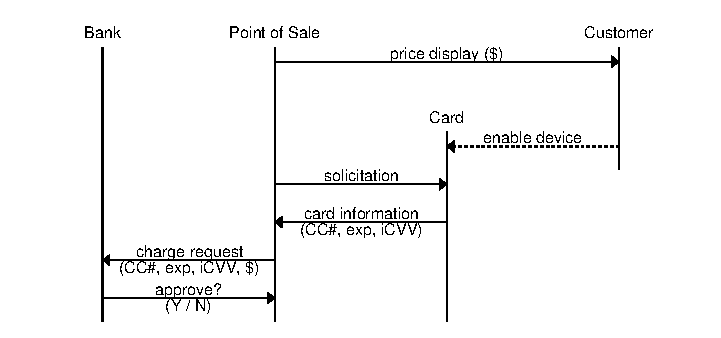
\includegraphics{img/insecure_ccp.eps}
  \label{fig:insecure-ccp}
\end{figure}

The message contents in the Insecure CC Protocol are as follows:

\begin{description}

\item[Solicitation:]
In practice, the solicitation message actually consists of a number of messages sent in both directions.
The purpose of these messages is to exchange information about the Credit Card type (e.g. \emph{Visa Credit}) and the Point of Sale model (e.g. \emph{2PAY.SYS.DDF01}), which defines the format of subsequent messages.
It is a choreographed dance with a specific (and constant) set of messages for a given model of Point of Sale and Credit Card, so we abstract this conversation to a single solicitation message.

\item[Card Information:]
This message contains all information necessary to coordinate an arbitrary charge request to the Credit Card's issuing Bank. It consists of four components:
\begin{itemize}
	\item The Credit Card number, identical to the number printed on the front of the card.
	\item The Credit Card's expiration date.
	\item An \emph{iCVV} (``integrated Card Verification Value'').
		This iCVV is a security code, similar to the 3-digit number printed on the back of a credit card, but is newly generated for each transaction.
		It is an element in a pseudo-random sequence generated by a secret seed known only to the Credit Card and its issuing Bank, making it unpredictable to third parties.
	\item The issuing Bank name.
		This field is used for routing purposes, and is not a component of the subsequent charge request.
		As such, it is not pictured in Figure \ref{fig:insecure-ccp}.
\end{itemize}

\item[Charge Request:]
This message is sent to the Bank identified in the card information message, and consists of four components:
\begin{itemize}
	\item The Credit Card number, identifying the account to be charged.
	\item The Credit Card's expiration date.
	\item The Credit Card's iCVV.
	\item The dollar amount to be charged.
\end{itemize}

\item[Approval:]
This message consists of a \emph{response code} determined by the Bank, indicating its decision relating to the charge request.
The bank makes this decision after verifying the information supplied in the charge request message, and performing additional checks such as matching the purchase to a known location of the Customer.
The most common response codes are the result of a simple approval decision (i.e. ``Approved'' or ``Declined''),
although a number of different codes (e.g. ``Pick up card'' if the card was reported lost or stolen, etc.) are also supported.
We abstract this message as a single bit: whether or not the Customer's account has been charged.

\end{description}

\section{Attacks on the Protocol}
\label{sec:insecure-attacks}

The Insecure CC Protocol is vulnerable to a number of attacks that can be performed by an external adversary.
We classify these attacks into four broad categories:
    eavesdropping, skimming attacks, relay attacks, and attacks facilitated by compromised points of sale.
In this section, we describe these attacks in detail.


\subsection{Eavesdropping}
\label{sec:insecure-eavesdropper}
The goal of an eavesdropper is to gain the victim's credit card number and expiration date.
Eavesdropping is a passive attack, where the eavesdropper hears all communication between the point of sale and the credit card.
(Communication between the Cank and the point of sale is securely transmitted over the Internet.)
An outline of this attack is shown in Figure \ref{fig:insecure-eavesdropper}.

\begin{figure}
  \caption{Eavesdropping}
  \centering
    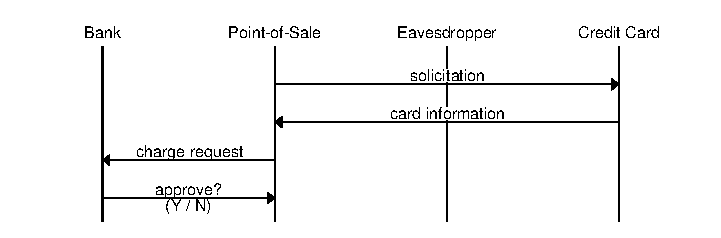
\includegraphics{img/attack-3-eavesdrop.eps}
  \label{fig:insecure-eavesdropper}
\end{figure}

We have demonstrated the feasibility of this attack by building a very low form-factor antenna capable of eavesdropping on NFC communications.
Similar to the device described in \cite{kortvedt2009eavesdropping}, we modified a MIFARE NFC tag to act as an antenna by disabling the chip at the center and attaching leads to either side of the coil where they connect to the chip.
We then measure the voltage induced in the coil.

In Figure \ref{fig:insecure-eavesdropper-antenna}, we show our NFC eavesdropping antenna next to a credit card for scale.
The resulting antenna is paper thin, flexible, approximately 3cm in diameter and adhesive on one side.
As such, it can easily be concealed within range of a point of sale.

\begin{figure}
  \caption{Eavesdropping Antenna (credit card for scale)}
  \centering
    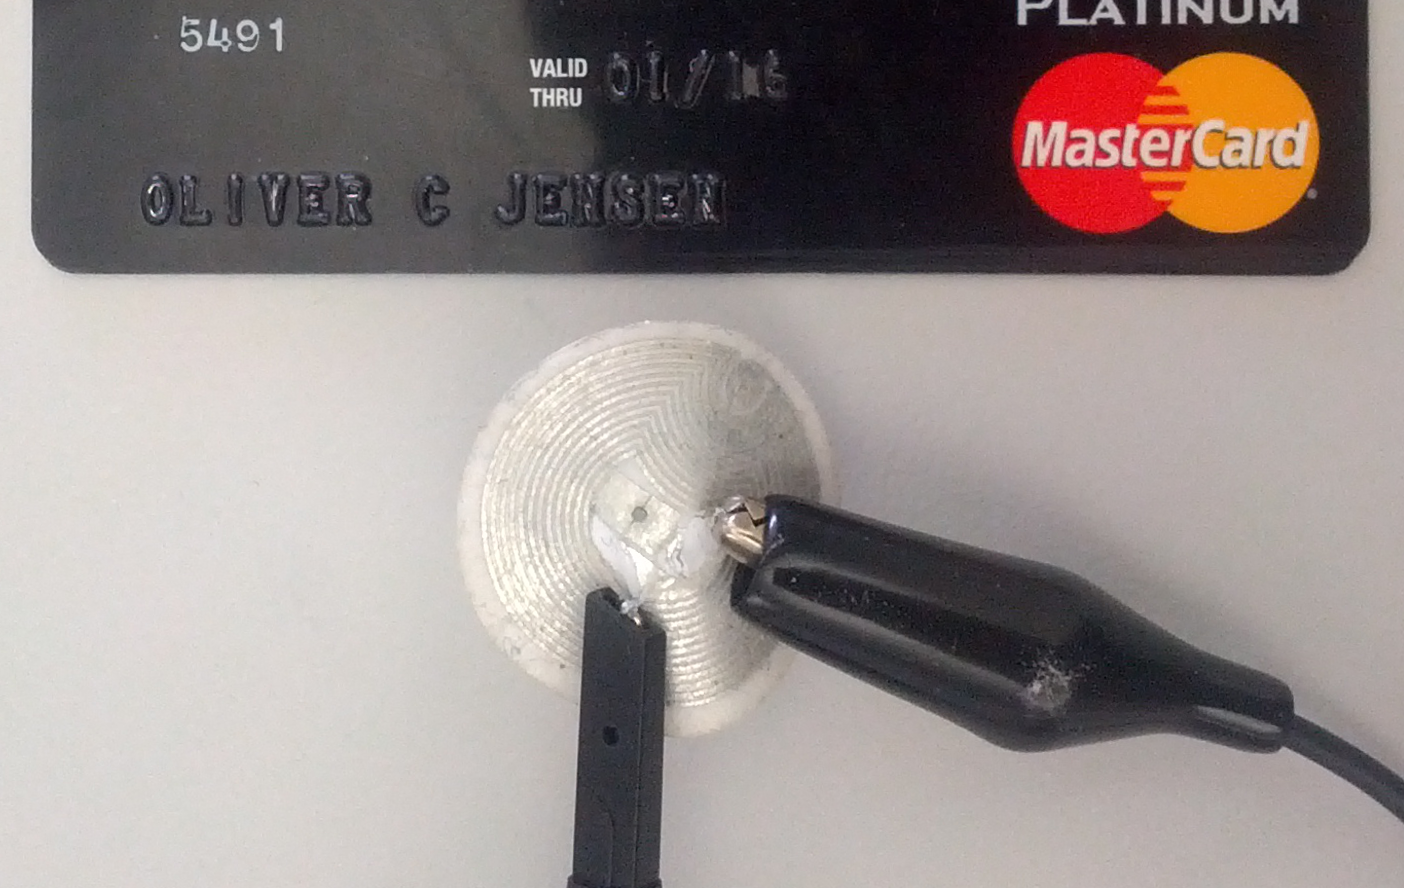
\includegraphics[width=1.0\textwidth, clip=true, trim=0 0 0 0]{img/attack-3-eavesdrop-photo.png}
  \label{fig:insecure-eavesdropper-antenna}
\end{figure}

By connecting such a makeshift antenna to a software-defined radio (available very inexpensively online) and recording the captured signal with a program like GNU Radio, an eavesdropper can record all transmissions that occur between the point of sale and credit cards.
We have written a simple program to read these signal-recordings and decode the messages in each direction.

In the Insecure CC Protocol, an eavesdropper acquires the credit card number, expiration date and the issuing bank name.
(The eavesdropper also acquires the iCVV, but since this is used immediately in the current transaction, the acquired iCVV is of no value.)





\subsection{Skimming}
\label{sec:insecure-skimmer}
The goal of a skimmer is to perform a purchase on behalf of the victim, without the victim's knowledge or consent.
First, the skimmer masquerades as a point of sale to the victim's credit card, acquiring the credit card number, expiration date, issuing bank name, and the next iCVV.
Subsequently, the skimmer masquerades as a credit card to a legitimate point of sale, making a purchase on behalf of the victim by replaying the skimmed credit card information and the iCVV.
An outline of this attack is shown in Figure~\ref{fig:insecure-skimmer}.

\begin{figure}
  \caption{Skimming}
  \centering
    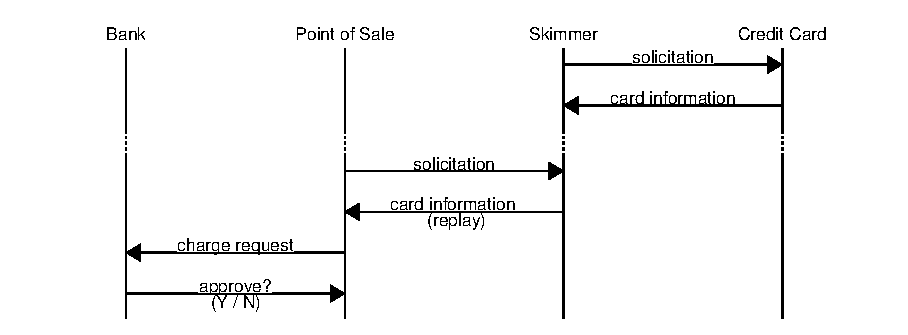
\includegraphics{img/attack-3-skim.eps}
  \label{fig:insecure-skimmer}
\end{figure}

This attack can be performed using a smart-phone with NFC capabilities.
An Android application called \emph{NFCProxy}\footnote{\emph{NFCProxy}\cite{NFCProxy}, presented at Defcon 20, can be downloaded here: \url{http://sourceforge.net/projects/nfcproxy/}} automates this attack, and is freely available online.
While \emph{NFCProxy} is not listed in the Google Play store, it can be downloaded from SourceForge and installed on the phone in a matter of minutes.

With \emph{NFCProxy} running, the skimmer brings his phone briefly within range of an NFC credit card to acquire the credit card information and  the iCVV.
When the skimmer wishes to perform the illegitimate purchase on behalf of the victim, the skimmer moves their phone within range of a point of sale as though it were a credit card.

In the Insecure CC Protocol, a skimmer may perform a single purchase (limited by the lack of subsequent iCVVs).
The skimmer must take care to perform this purchase before the credit card holder makes a purchase of their own, as this would invalidate the skimmed iCVV.
(The skimmer also gains all information that an eavesdropper would learn.)






\subsubsection{Relay Attacks}
\label{sec:insecure-relay}

Much like the skimmer, the goal of the relay attacker is to perform purchases on behalf of the victim, without the victim's knowledge or consent.
Multiple devices may be used to relay skimmed credit card information across a separate channel, effectively breaking down the assumption of proximity built into NFC.
This attack can also be performed using the \emph{NFCProxy} Android application, described in Section \ref{sec:insecure-skimmer}.
An outline of this attack is shown in Figure \ref{fig:insecure-relay}.

\begin{figure}
  \caption{Relay Attack}
  \centering
    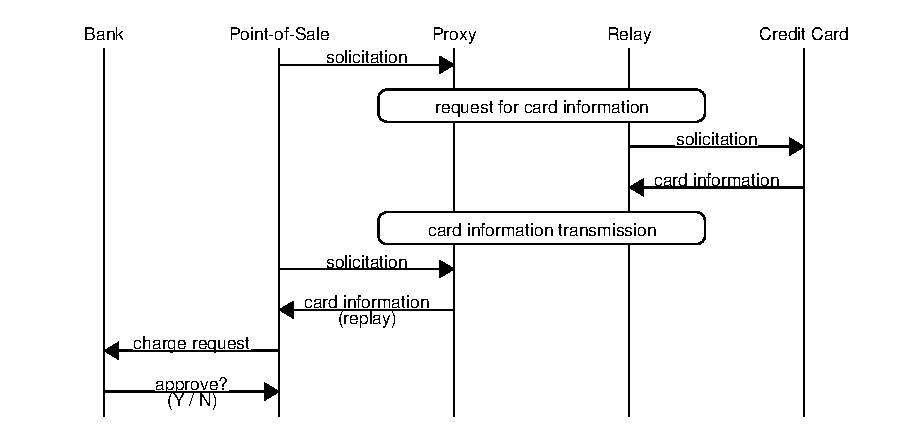
\includegraphics{img/attack-3-relay.eps}
  \label{fig:insecure-relay}
\end{figure}

In implementation, a relay attack is very similar to a skimming attack, with the exception that the skimmer is separated into two entities, called ``proxy'' and ``relay''.
These two entities are spatially disparate, but are connected through an out-of-band communication channel.
The relay positions his phone near the victim's credit card, while the proxy approaches a point of sale.
Whenever the proxy is ready to make a purchase, it sends a message to the relay requesting fresh values from the victim's credit card.

The relay skims the credit card, and forwards the card's information back to the proxy, enabling it to make a purchase on behalf of the victim.
These messages may be transmitted over any communication channel, but are most easily sent over a wireless LAN.

In the Insecure CC Protocol, a proxy may perform multiple purchases if the relay remains in proximity of the victim's credit card, querying it for fresh iCVVs for every purchase.





\subsubsection{Attacks Facilitated by Compromised Points of Sale}
\label{sec:insecure-compromised}

The Insecure CC Protocol implicitly trusts the ability of a retailer to keep its data secure.
By allowing persistent sensitive information (e.g. the credit card number and expiration date) to be transmitted to a device under the retailer's control,
  this protocol invites attacks on the retailer's own systems.
We use this category of attacks to refer to any attacks which involve the point of sale or merchant performing (possibly unintentional) actions leading to credit card theft\footnote{
	In the Compromised point of sale model we consider only devices which correctly adhere to the protocol.
	We explicitly exclude what we term \emph{malicious} points of sale, those which may perform arbitrary actions such as refusing to randomize random values, etc.
	Defending against a malicious point of sale in any payment setting is much more involved, and is discussed later.
}.
For example, a point of sale might be compromised and re-programmed to transmit credit card information to an attacker after every successful purchase.
An outline of this attack is shown in Figure~\ref{fig:insecure-compromised}.

\begin{figure}[h!]
  \caption{Compromised Point of Sale}
  \centering
    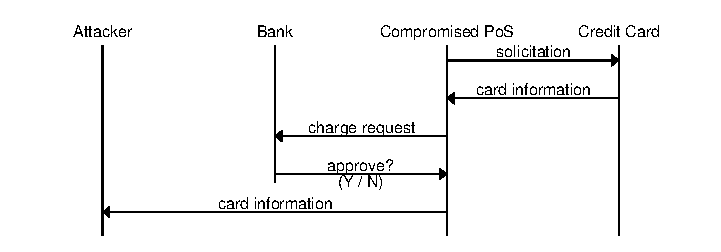
\includegraphics{img/attack-3-comppos.eps}
  \label{fig:insecure-compromised}
\end{figure}

The compromise of points of sale is far from a theoretical threat:
these attacks have become alarmingly commonplace, to the point that they have been covered by mainstream news sources including the New York Times \cite{neimanmarcushack} and the Wall Street Journal \cite{targethack}\cite{homedepothack}.

In November through December 2013, unauthorized access was gained to an estimated 40,000 points of sale used by U.S. retailer Target.
This data breach was widely publicized, as it resulted in the compromise of \emph{40 million} credit and debit cards, and other personal information of 70 million customers as reported in the Wall Street Journal \cite{targethack}.

More recently, in September 2014, Home Depot confirmed a similar data breach.
According to subsequent investigations, it appears that the same malware as was used against Target was at the heart of the Home Depot breach.
During this breach, attackers stole \emph{56 million} credit and debit cards, also as reported in the Wall Street Journal \cite{homedepothack}.

Other recent victims of Compromised points of sale include other retailers
	(e.g. Neiman Marcus in July through October of 2013, in which attackers stole an estimated 1.1 million credit and debit cards)\cite{neimanmarcushack},
	grocery stores (e.g. Supervalu in June through July of 2014, in which it is estimated that attackers stole ``millions'' of credit and debit cards\cite{supervaluhack}),
	as well as restaurants (e.g. P.F. Chang's in September 2013 through June 2014, in which attackers stole an estimated 7 million credit and debit cards\cite{pfchanghack}).

Since 2014, headlines regarding data theft from compromised points of sale have diminished,
    not because the attacks have slowed, but because they have become so prevalent they are no longer headline-worthy.


\chapter{The Externally Secure CC Protocol}
\label{cha:external}
In Chapter 2 we described the protocol in use today for contactless credit card payments,
    and showed that this protocol is vulnerable to four types of external attacks.
In this chapter, we show how to modify the protocol in order to defend against these attacks.
This modified protocol is called the Externally Secure CC Protocol

\section{Goals of the Protocol}
\label{sec:external-goals}

The Externally Secure CC Protocol has two goals.
First, this protocol should defend against the four types of attacks:
    eavesdropping, skimming, relay attacks, and attacks facilitated by compromised Points of Sale.
Second, we construct this protocol to minimize the computation which occurs on the card itself.

Contactless credit cards today are capable of only very limited computation, and do not engage in any cryptographic operations.
We hypothesize that the limited computaional power on credit cards is to reduce costs to a minimum:
	credit cards must be disposably cheap to manufacture, so that they can be immediately replaced on suspicion of compromise.

\section{Design of the Protocol}
\label{sec:external-design}

In designing the Externally Secure CC Protocol, we do not add any computationally expensive operations such as signature verification, or even hashing on the credit card:
    beyond its current function, we restrict a credit card to performing only basic arithmetic, indexing, XOR, and similarly inexpensive operations.
We design the protocol using a process called \emph{stepwise refinement}:
\begin{enumerate}
\item First, we define the protocol in terms of an abstract function \emph{H}.
\item We then identify two desired properties of function \emph{H}, namely \textbf{H1} and \textbf{H2},
	and show that if function \emph{H} satisfies these two properties,
	then the protocol is not vulnerable to the four classes of attacks described in Section \ref{sec:insecure-attacks}.
\item Next, we define function \emph{H} in terms of two abstract functions \emph{F} and \emph{G}.
We then identify three properties, namely \textbf{F1}, \textbf{F2}, and \textbf{G1},
	and prove that if function \emph{F} satisfies properties \textbf{F1} and \textbf{F2}
	and function \emph{G} satisfies property \textbf{G1}, then function \emph{H} satisfies the two desired properties \textbf{H1} and \textbf{H2}.
\item We then propose concrete implementations of functions \emph{F} and \emph{G}.
\item Finally, we argue that our proposed implementation of function \emph{F} satisfies properties \textbf{F1} and \textbf{F2},
	and that our proposed implementation of function \emph{G} satisfies property \textbf{G1}.
\end{enumerate}

In so doing, we provide a concrete implementation of the Externally Secure CC Protocol
	and show that it is not vulnerable to any of the four classes of outsider attacks described in Section \ref{sec:insecure-attacks}.

The Externally Secure CC Protocol uses the same four messages that are used in the Insecure CC Protocol.
However, the contents of these messages have become more involved.
In particular, we incorporate a challenge-response mechanism in the Solicitation and Card Information messages.
An outline of this protocol is shown in Figure \ref{fig:external-ccp}.

\begin{figure}[h!]
  \caption{Externally Secure CC Protocol}
  \centering
    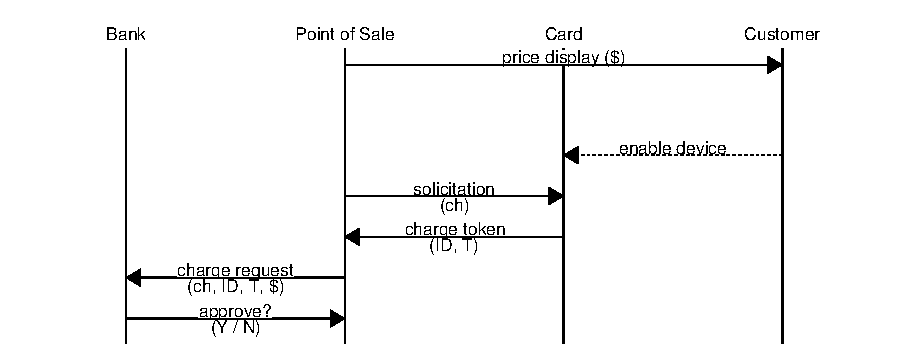
\includegraphics{img/external_ccp.eps}
  \label{fig:external-ccp}
\end{figure}

The four messages used in the Externally Secure CC Protocol are as follows:

\begin{description}
\item[Solicitation (\emph{ch}):]
The point of sale sends a Solicitation message much like in the Insecure CC Protocol.
However, this message now includes a random challenge \emph{ch}.
This challenge is used by the credit card when constructing its response.

\item[Card Information (\emph{ID}, \emph{T}):]
The credit card's response consists of two primary components, ID and T. They are as follows:

\begin{description}
\item[\emph{ID},]a Universally Unique Identifier \cite{uuid}, is used to identify the card without revealing the card's information to eavesdroppers or any other party.
This value is computed by the credit card manufacturer and stored on the card as a constant.

\item[\emph{T = H(info, ch, iCVV)}] is used to authenticate the card's identity.
This abstract function \emph{H} will be defined later through stepwise refinement, but informally we can think of it as similar to a cryptographic hash function:
	it can be used to verify its arguments while leaking no information about them.
\end{description}

In so doing, \emph{ID} provides identification and \emph{T} provides authentication.
In addition, this message is accompanied by the bank name \emph{B}, as before, so that the point of sale may route its Charge Request to the proper entity.

\item[Charge Request (\emph{ID}, \emph{T}, \emph{ch}, \emph{\$}):]
After receiving the Card Information message, the point of sale issues a Charge Request to the credit card's issuing bank.
The point of sale does not learn the card's private information, but simply forwards the card identification (\emph{ID}) and authentication (\emph{T}) to the bank \emph{B},
    specified in the Card Information message.
The point of sale also includes the challenge \emph{ch}
	(so that the bank can verify that \emph{T} is a valid response to \emph{ch} from card \emph{ID}),
	as well as the dollar amount to be charged.

\item[Approval (Y/N):]
The bank maintains an index of \emph{ID} into its account database.
When the bank receives a Charge Request message, it identifies the matching record as specified by \emph{ID}, looking up $\textrm{\emph{info}}_{bank}$ and $iCVV_{bank}$.
It then calculates $T_{bank} = H(\textrm{\emph{info}}_{bank},~ ch,~ iCVV_{bank})$ and verifies that $T = T_{bank}$.
This step is equivalent to verifying the credit card information and iCVV in the Insecure CC Protocol,
	and results in a decision to accept or reject the charge request.

\end{description}





\subsection{Desired Properties of Function \emph{H}}
\label{external-h-properties}

We pit the Externally Secure CC Protocol against the attacks described in Section \ref{sec:insecure-attacks}
	and identify the two properties \textbf{H1} and \textbf{H2} needed from function \emph{H} in order for these attacks to be thwarted.

\subsubsection*{Defending Against Eavesdropping}
When eavesdropping on a transaction, the eavesdropper learns a valid (\emph{ch}, \emph{ID}, \emph{T}, \emph{B}) tuple.
The challenge \emph{ch}, the card identifier \emph{ID}, and the bank name \emph{B} are all public information, of no value to the eavesdropper.
Only $T = H(\textrm{\emph{info}},~ ch,~ iCVV)$ contains authentication information useful to an eavesdropper.
In order to guarantee that no sensitive information is leaked, we require that function \emph{H} satisfies the following property:

\begin{description}
\item[H1:] If \emph{iCVV} is indistinguishable from random, then $H(\textrm{\emph{info}},~ ch,~ iCVV)$ is indistinguishable from random.
\end{description}

If function \emph{H} satisfies property \textbf{H1}, then the eavesdropper (ignorant of \emph{iCVV}) cannot distinguish \emph{T} from random and gains no useful information.








\subsubsection*{Defending Against Skimming}
When sending a Solicitation message to a credit card, the skimmer includes a challenge $ch_{skim}$, which the card uses to construct its response.
From the resulting Card Information message, the skimmer learns \emph{ID}, $T_{skim} = H(\textrm{\emph{info}}, ch_{skim}, iCVV)$ and \emph{B}.
When the skimmer attempts to perform a purchase using this information, it will be issued a challenge $ch_{pos}$ by the point of sale.
In order to prevent the skimmer from correctly responding to this challenge, we require that function \emph{H} satisfies the following property:

\begin{description}
\item[H2:] Given $H(\textrm{\emph{info}},~ ch,~ iCVV)$, \emph{ch}, and $ch'$ such that $ch \neq ch'$, one cannot infer $H(\textrm{\emph{info}},~ ch',~ iCVV)$.
\end{description}

If function \emph{H} satisfies property \textbf{H2}, then the skimmer cannot use the value of $T_{skim}$ in order to construct a response to the point of sale's challenge $ch_{pos}$, and thus cannot perform purchases on behalf of the credit card.






\subsubsection*{Defending Against Relay Attacks}
The relay attack operates similarly to the skimming attack.
When performing a relay attack, the relay provides challenge $ch_{relay}$ to the card.
As in the skimming attack, the relay learns \emph{ID}, $T_{relay} = H(\textrm{\emph{info}},~ ch_{relay},~ iCVV)$, and \emph{B}, and then transmits this information to the proxy.
When the proxy attempts to perform a purchase, it is issued a challenge $ch_{pos}$ by the point of sale.

Thus, if function \emph{H} satisfies the property \textbf{H2},
	then the proxy cannot use the value of $T_{relay}$ in order to construct a valid response to the point of sale's challenge $ch_{pos}$,
	and as a result, cannot perform this purchase on behalf of the credit card.






\subsubsection*{Defending Against Compromised Points of Sale}
A compromised point of sale will result in an attacker learning a valid (\emph{ch}, \emph{ID}, \emph{T}, \emph{B}) tuple,
	which the point of sale requires in order to construct a Charge Request message.
Note that this is the same information learned by the attacker in the eavesdropping case.
As such, if the function \emph{H} satisfies property \textbf{H1}, then the information learned by a compromised point of sale is of no value:
	no private information about the credit card is leaked,
	and the authentication token \emph{T} cannot be reused since the \emph{iCVV} used in its construction is no longer valid after the charge has occurred.



In summary, in order to defend against the four classes of attacks described in Section \ref{sec:insecure-attacks},
	we require that the \emph{iCVV} be a pseudorandom value, and that function \emph{H} upholds the following two properties:

\begin{description}
\item[H1:] If \emph{iCVV} is indistinguishable from random, then $H(\textrm{\emph{info}},~ ch,~ iCVV)$ is indistinguishable from random.
\item[H2:] Given $H(\textrm{\emph{info}},~ ch,~ iCVV)$, \emph{ch}, and $ch'$ such that $ch \neq ch'$, one cannot infer $H(\textrm{\emph{info}},~ ch',~ iCVV)$.
\end{description}









\subsection{Implementing Function \emph{H}}

We find it convenient to define function \emph{H} as a composition of functions \emph{F} and \emph{G} as follows:

$H(\textrm{\emph{info}},~ ch,~ iCVV) = F(x,~ iCVV) \textrm{ where } x = G(\textrm{\emph{info}},~ ch)$

Once defined in these terms, we posit the properties \textbf{H1} and \textbf{H2} in terms of functions \emph{F} and \emph{G}.
We then show that if function \emph{F} satisfies the properties \textbf{F1} and \textbf{F2}, and function \emph{G} satisfies the property \textbf{G1},
then function \emph{H} satisfies the desired properties \textbf{H1} and \textbf{H2}.

\begin{description}
\item[F1:] If $y$ is indistinguishable from random, then $F(x, y)$ is indistinguishable from random.
\item[F2:] Given only $x$, or given only $y$, one cannot infer $F(x, y)$.
\item[G1:] Given $G(u, v)$, $v$, and $v'$ such that $v \neq v'$, one cannot infer $G(u, v')$ without knowledge of $u$.
\end{description}

\newtheorem{theorem}{Theorem}

\begin{theorem}
If function \emph{F} satisfies property \textbf{F1}, then function \emph{H} satisfies property \textbf{H1}.
\end{theorem}

\begin{proof}
  Let $x = G(\textrm{\emph{info}},~ ch)$ for any $\textrm{\emph{info}}$,~ $ch$.
  Then $H(\textrm{\emph{info}},~ ch,~ iCVV) = F(x,~ iCVV)$.
  Thus if $y = iCVV$ is indistinguishable from random, then by property \textbf{F1}, $F(x,y) = H(\textrm{\emph{info}},~ ch,~ iCVV)$ is indistinguishable from random.
\end{proof}


\begin{theorem}
If function \emph{F} satisfies property \textbf{F2}, and function \emph{G} satisfies property \textbf{G1}, then function \emph{H} satisfies property \textbf{H2}.
\end{theorem}

\begin{proof}
  Let $x = G(\textrm{\emph{info}},~ ch)$ and $x' = G(\textrm{\emph{info}},~ ch')$ for any $\textrm{\emph{info}}$.
  By property \textbf{F2}, evaluating $H(\textrm{\emph{info}},~ ch',~ iCVV)$ requires knowledge of $x' = G(\textrm{\emph{info}},~ ch')$.
  However, by property \textbf{G1}, one cannot infer $G(\textrm{\emph{info}},~ ch')$ without knowledge of $\textrm{\emph{info}}$.
  Further, by property \textbf{H1}, no bits of $\textrm{\emph{info}}$ are leaked and thus $\textrm{\emph{info}}$ remains secret.
  Thus, given $H(\textrm{\emph{info}},~ ch,~ iCVV)$, $ch$, and $ch'$ such that $ch \neq ch'$, one cannot infer $H(\textrm{\emph{info}},~ ch',~ iCVV)$.
\end{proof}

While $\textrm{\emph{info}}$ is considered secret, it cannot be used directly in function \emph{G}.
This is because while most of the data in $\textrm{\emph{info}}$ is unpredictable, many of the bits are not random.
For example, in a typical credit card number, the first six digits are taken from the \emph{Issuer Identification Number}, a public value assigned to the issuing bank.
Similarly, the attacker can guess the bytes representing the expiration month and year from a very small set of possibilities.
Furthermore, the credit card number and expiration date are transmitted as decimal values transliterated into hexadecimal (e.g. ``4491'' is transmitted as two bytes: \texttt{0x44} and \texttt{0x91}).
As such, inferences may be made about the value of particular bits, since each such byte is drawn from only 154 possible values.

To resolve this problem, we use a keyed hash function known as an HMAC \cite{krawczyk1997hmac} to compute $h_k(\textrm{\emph{info}})$, using a key \emph{k} known only to the bank.
As \emph{info} does not change over the lifetime of the credit card, $h_k(\textrm{\emph{info}})$ is stored as a constant on the card.
As such, the computation necessary for hashing is not executed on the credit card, and the card requires no knowledge of the bank's secret key \emph{k}.
For convenience we will refer to the output of $h_k(\textrm{\emph{info}})$ as the constant \emph{khi}.

We propose implementations for functions \emph{G} and \emph{F} (and thus \emph{H}) in Figure \ref{fig:implementation}.
Note that function \emph{G} is defined as the function which returns those bits of a keyed HMAC $h_k(\textrm{\emph{info}})$ for which the corresponding bit of $ch$ was set to 1.
Also note that function \emph{F} is defined as \texttt{XOR}.

\begin{figure}[h!]
  \caption{Implementation of \emph{F}, \emph{G} and \emph{H}}
  \begin{verbatim}

function G(info, ch):
    const khi = HMAC(bank_key, info)
    result = empty list of bits
    for each of the n bits of ch:
        if the n'th bit of ch is 1:
            append n'th bit of khi to result
    return result

function F(x, iCVV):
    return x XOR iCVV

function H(info, ch, iCVV):
    x = G(info, ch)
    return F(x, iCVV)
\end{verbatim}
  \label{fig:implementation}
\end{figure}

In the Insecure CC Protocol, $\textrm{\emph{info}}$ is composed of 96 bits, and $iCVV$ is composed of 32 bits.
If we maintain these field-lengths in the Externally Secure CC Protocol, and use an HMAC function which also outputs 96 bits, then our implementation of \emph{F} and \emph{G} requires that $ch$ must be a 96 bit value with 32 1's and 64 0's.
More generally, our implementation requires that $h_k(\textrm{\emph{info}})$ and $ch$ have the same number of bits,
	and that the number of \emph{1-bits} in \emph{ch} is equal to the number of bits in \emph{iCVV}.

Note that the \texttt{XOR} operation satisfies properties \textbf{F1} and \textbf{F2}, so our implementation of function \emph{F} (trivially) satisfies them as well.

The output of $G(\textrm{\emph{info}},~ ch)$ is composed of a number of bits of \linebreak $\textrm{\emph{khi}} = h_k(\textrm{\emph{info}})$ selected by the challenge $ch$.
If $ch_1 \neq ch_2$, one cannot infer $G(khi,~ ch_2)$ from $G(khi,~ ch_1)$ without knowledge of $khi$,
because the results are composed of different bits of $khi$ selected by the challenges $ch_1$ and $ch_2$.
These bits are indistinguishable from random to any party without knowledge of $\textrm{\emph{info}}$ and the bank's secret key $k$.
These bits are then masked by the $iCVV$ and as such are not learned by any party.
As a result, our implementation of function \emph{G} satisfies the property \textbf{G1}.


\chapter{The Secure CC Protocol}
\label{cha:secure}
The Externally Secure CC Protocol described in Chapter \ref{cha:external} focuses on defending the retailer and customer from malicious external parties, termed ``outsiders''.
In this chapter, we examine the problems posed by malicious retailers and focus on how to secure contactless credit cards against them.
As will be described shortly, attacks by malicious retailers are particularly pernicious, as they are less easily identified as fraud.
Even when these attacks are detected, the resolutions are not always simple.\footnote{
        Portions of this chapter have previously been published in \cite{jensen2}.
        While most of the contributions in this chapter are my own,
        acknowledgements are due to Tyler O'Meara for suggesting that the Transparent Bridge attack could be applicable to contactless credit cards,
        and to Mohamed Gouda for helping construct clear and concise protocol descriptions.
}

\section{Goals of the Protocol}
\label{sec:secure-goals}

Recall that when making a payment, the customer first views the price about to be charged on the screen of the retailer's point of sale.
Using this information, the customer makes his one and only decision: whether to allow the payment protocol to occur, or not.
The underlying assumption that the customer makes is that the price displayed on the screen is equal to the price which will be charged to his credit card.
This need not be the case: the information displayed on a screen is merely an assurance in the informal sense:
	the numbers displayed to the customer \emph{should} reflect the dollar amount which will subsequently be sent with the Charge Request message to the bank,
    but there is no mechanism in place to require this.
Two attacks emerge as a result.
The goal of the Secure CC Protocol presented in this chapter is to extend the protection provided by the Externally Secure CC Protocol to defend against these two attacks.

\subsection{The Over-charge Attack}
\label{sec:overcharge}
An Over-charge attack, illustrated in Figure \ref{fig:attack_overcharge}, is characterized by the malicious point of sale displaying one price to the customer
	and then sending a higher price to the bank
	(in the Charge Request message of the CC Protocols).
As a result, the customer believes himself to have been charged one amount, but is instead charged an arbitrarily higher amount.
Since the customer is uninvolved in the protocol besides the initial step of allowing the protocol to occur,
	there is no mechanism ensuring that the price displayed to the customer matches the price that the (malicious) point of sale sends to the bank.

\begin{figure}
  \caption{Over-charge Attack}
  \centering
    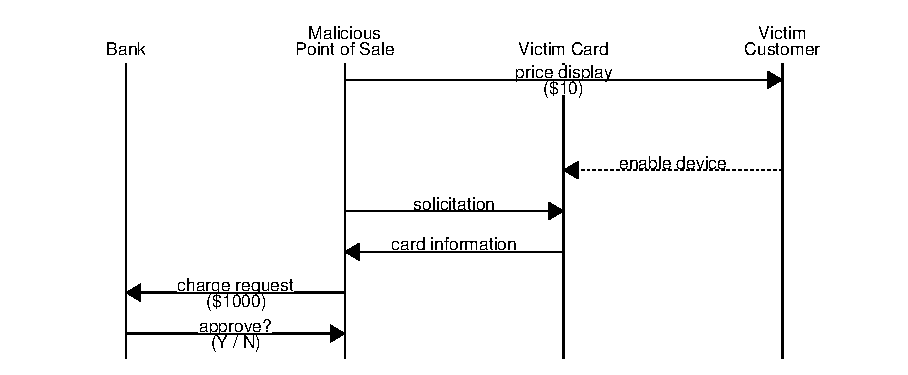
\includegraphics{img/attack-mr-overcharge.eps}
  \label{fig:attack_overcharge}
\end{figure}

Should a customer become aware of an over-charge when reviewing his monthly statement, he may file a charge-back request with his bank, nullifying the payment as fraudulent.
As a result, while the amount by which the customer may be overcharged is unconstrained by the protocol, it should be relatively small for the attack to ultimately be successful.
For example, it is easy to notice a gas station charge for \$500.00 instead of \$21.87 on a monthly statement, and the resulting investigation would be uncomplicated.
However, should the struggling business choose to increase charges by 5\%, the resulting gas station charge of \$22.96 could very easily be overlooked.
Even were it to be noticed, the victim customer may have difficulty proving the discrepancy.


\subsection{The Transparent Bridge Attack}
\label{sec:transparent-bridge}
A more interesting attack is described by Drimer and Murdoch \cite{Drimer:2007:KYE:1362903.1362910}.
The authors consider a man-in-the-middle attack, perpetrated by a malicious retailer and an accomplice with specialized equipment.
This attack involves four parties: a victim customer, a malicious retailer, a malicious customer, and a victim retailer.
The malicious retailer and the malicious customer collude to perform this attack.

The malicious customer is issued with a special device, capable of relaying all messages it receives from a point of sale to the malicious retailer in real time.
Similarly, it can relay any responses it receives from the malicious retailer back to this point of sale.
As a result, the malicious customer and malicious retailer can together form a bridge between the victim credit card and the victim retailer's point of sale.
The attack is illustrated in Figure \ref{fig:attack_bridge} and runs as follows:

\begin{enumerate}
\item First, the victim customer attempts to make a relatively inexpensive purchase from the malicious retailer.
Simultaneously, the malicious customer prepares to make a relatively expensive purchase from a victim retailer.
\item The victim retailer's point of sale issues a Solicitation message to the malicious customer, who relays it to the malicious retailer.
\item The malicious retailer then forwards this Solicitation message to the victim credit card.
\item The victim credit card responds with a Card Information message to the malicious point of sale, who relays this message to the malicious customer.
\item The malicious customer forwards this Card Information message to the victim retailer's point of sale.
\item The victim retailer's point of sale issues a Charge Request message to the victim credit card's bank, charging the victim customer for the expensive purchase.
\end{enumerate}

\begin{figure}
  \caption{Transparent Bridge Attack}
  \centering
  	\hspace*{-0.35in}
    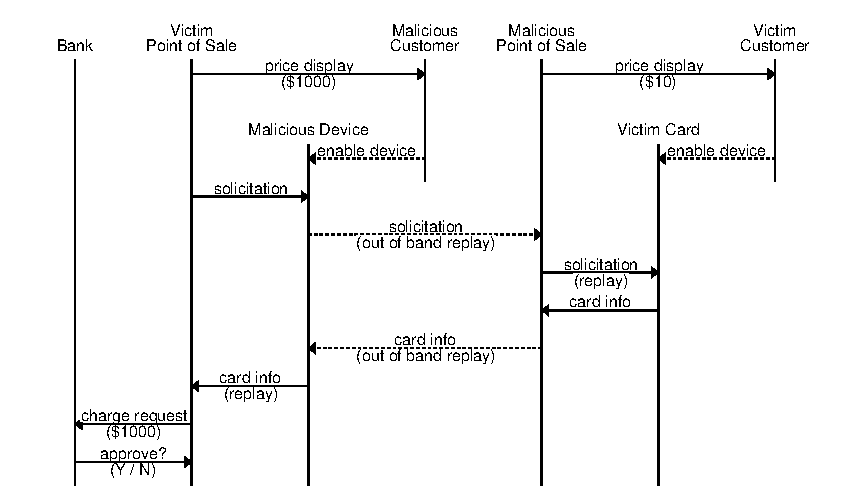
\includegraphics{img/attack-mr-bridge.eps}
  \label{fig:attack_bridge}
\end{figure}

In this attack, all messages are transparently relayed between the victim retailer's point of sale and the victim customer's credit card.
As a result, the victim customer believes himself to be making an inexpensive purchase at the malicious retailer, while he is actually making an expensive purchase at the victim retailer.
The malicious retailer loses the inexpensive sale, but acquires the merchandise from an expensive purchase in exchange.

This Transparent Bridge attack is particularly interesting, because the malicious parties leave no trace with either of the victims:
to the victim customer there is only a record of an expensive purchase at the victim retailer, and to the victim retailer there is only the customer record of the victim customer.
The amount which can be successfully stolen by the malicious retailer is unconstrained, and needs not evade notice:
	if the discrepancy is noticed and the victim customer files a charge-back request, it will be against the victim retailer (and not the malicious retailer).
As such, detected or not, it is one of the two victims that will be left facing the bill, making the Transparent Bridge attack significantly more dangerous than the Over-charge attack described earlier.

Drimer et al. propose a defense against this attack in the context of EMV credit cards (colloquially known as ``chip and pin'').
However, this solution is not applicable to contactless credit cards.

\section{Design of the Protocol}
\label{sec:secure-design}

Since the attacks described in the previous section (allowing a malicious retailer to exploit a customer)
	are tied to the retailer's ability to display one price and charge another,
	our proposed defense against these attacks is built around removing this ability.
If using a credit card implemented on a smart phone, the phone's interface provides an additional communication channel between the customer and the credit card.
In this case we refer to the card as a ``virtual'' credit card.
The communication channel between the smart phone and the customer can be harnessed to allow the customer to participate in the credit card protocol,
	beyond simply allowing it to occur.

The Externally Secure CC Protocol described in Chapter \ref{cha:external} defines a function \emph{H},
    proves several of its properties, and uses it to defend against external attacks such as skimming and eavesdropping.
We note that each property required of this function \emph{H} is a property enjoyed by common cryptographic hash functions,
    such as those in the \emph{SHA} family.
As such, using a hash function instead of the derived function \emph{H} does not reduce the security of the Secure CC Protocol.
In the context of virtual credit cards, the computational cost of executing a hash function is no longer a concern.

We remind the reader of the following terms:

\begin{description}
\item[ch:] a fresh, randomly generated challenge value, chosen by the point of sale.
\item[info:] the credit card's payment information, consisting of the credit card number and expiration date.
\item[ID:] a UUID, uniquely identifying an individual credit card without revealing any information about \emph{info}.
	This identifier is stored as a constant on the credit card.
\item[iCVV:] an unpredictable value freshly generated by the credit card for each transaction (the issuing bank can generate the same sequence of values).
\item[B:] the name of the issuing bank, used for the purpose of routing transactions as before.
\item[T:] a charge token, to authenticate a single transaction.
\end{description}

The Secure CC Protocol, operating between a point of sale and a virtual credit card, is illustrated in Figure \ref{fig:secure-ccp} and proceeds as follows:

\begin{enumerate}
\item The point of sale displays a price \val{\$d} on its screen, inviting the customer to bring his credit card within NFC range.
\item The point of sale sends a Solicitation message to the credit card, including a fresh random challenge \val{ch} and the price to be charged \val{\$s}.
	(Recall that if the point of sale is honest, \val{\$s} = \val{\$d})
\item The virtual credit card displays the price \val{\$s} on the smart phone to the customer, who can choose to accept or reject it.
	Rejecting the price aborts the protocol here.
\item If the price is accepted by the customer, the virtual credit card calculates
    $$T = H(\textrm{\emph{info}},~ ch,~ \textrm{\emph{\$s}},~ \textrm{\emph{iCVV}})$$
	and responds to the point of sale with a Card Information message consisting of (\val{ID}, \val{T}, \val{B}).
\item The point of sale sends a charge request message to the issuing bank (identified by \val{B}) consisting of (\val{ID}, \val{T}, \val{ch}, \val{\$r}).
	(Again, if the point of sale is honest, \val{\$r} = \val{\$d})
\item The bank uses \val{ID} to look up \emph{info\textsubscript{bank}} and then calculates \emph{iCVV\textsubscript{bank}}.
	It then uses the \val{ch} and \val{\$r} supplied in the charge request message to determine
	$$T_{bank} = H(\textrm{\emph{info}}_{bank},~ ch,~ \textrm{\emph{\$r}},~ \textrm{\emph{iCVV}}_{bank})$$
	If $T \neq T_{\text{bank}}$, the bank will decline the charge, otherwise it approves the charge for \val{\$r}.
\end{enumerate}

\begin{figure}
  \caption{Secure CC Protocol}
  \centering
    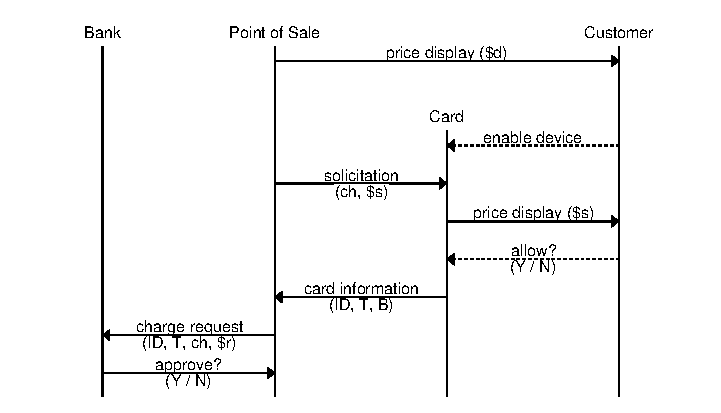
\includegraphics{img/secure_ccp.eps}
  \label{fig:secure-ccp}
\end{figure}

When using a physical credit card instead of a virtual one, no communication channel exists between the card and the customer.
As a result, the steps above in which the card displays the price sent with the Solicitation message (\val{\$s}) to the customer and waits for the customer to allow the protocol to proceed cannot occur.
Instead, a physical credit card must implicitly assume successful authorization from the customer, effectively skipping step 3.
As a result, while not providing protections from malicious retailers to physical credit cards, the protocol maintains backwards compatibility with no loss of functionality or security against malicious outsiders.

We note that a naive implementation of the protocol above might require excessively long timeouts between the point of sale sending its solicitation message and receiving the response.
Should long timeouts not be desired, a simple solution would be for the point of sale to send periodic solicitations (with new challenges).
The virtual credit card, upon receiving permission from the customer, could then cache this approval and respond immediately to the subsequent solicitation.
Besides noting this particular case, we emphasize that issues such as these are implementation details, the decisions for which are best left to those implementing the protocol.

\subsection{Defending Against the Over-charge Attack}

The Secure CC Protocol prevents the Over-charge attack against customers using a virtual credit card.
In step 3, the customer verifies that \linebreak \val{\$d} = \val{\$s} through visual comparison.
Due to the inclusion of \val{\$s} in the hash when generating token \emph{T}, we gain the assurance that for any charge accepted by the bank, \val{\$s} = \val{\$r}.

Thus, through a transitive argument, the customer can be assured that for any successful charge, \val{\$d} = \val{\$r}.
Should the malicious retailer attempt to issue a charge request with some $\textrm{\emph{\$r}} \neq \textrm{\emph{\$d}}$, then $T_{bank} \neq T$ and the charge will be declined by the bank.

\subsection{Defending Against the Transparent Bridge Attack}

The Secure CC Protocol makes no attempt to prevent this attack from occurring.
Instead, it removes the economic incentive of performing such an attack against customers using virtual credit cards.

In the Transparent Bridge attack, the malicious retailer loses the sale paid by the victim customer, in return for acquiring the purchase made by the malicious customer.
In order for the Transparent Bridge attack to be viable, the malicious actors must have something to gain:
  the value of the malicious customer's purchase must be greater than the value of the victim customer's purchase.
When the Secure CC Protocol is used, one of two scenarios occurs:

\begin{enumerate}
\item The price associated with the malicious customer's purchase differs from (i.e. is greater than) the price of the victim customer's purchase.
The victim customer compares the price displayed by the point of sale and the price displayed by his virtual credit card.
The would-be victim customer immediately detects the attack and aborts the transaction.
\item The price associated with the malicious customer's purchase is equal to the price of the victim customer's purchase.
The victim customer does not detect this attack, and allows the transaction to occur.
The end result: the victim customer paid for the price of what he received, and the victim retailer received the price of what it sold.
\end{enumerate}

As a result, there is no longer any incentive to carrying out this attack, as the only successful instance results in all parties getting paid exactly as much as they would had they been honest.


\chapter{Virtual Credit Cards and Electronic Wallets}
\label{cha:electronic}
When describing the Secure CC Protocol in Chapter \ref{cha:secure}, we referred to ``virtual credit cards''.
In this chapter, we describe them more formally.

\section{Virtual Credit Cards}

Many consumer smart phones today support the ability to communicate over the NFC channel.
Indeed, as described in Section \ref{sec:insecure-attacks}, this ability can be used by skimmers and relay attackers in order to perform fraudulent purchases.
Moreover, this ability can be used by an authorized party to perform non-fraudulent purchases.

A virtual credit card is an application on an NFC-capable smart phone, which emulates a credit card in a CC Protocol,
    by receiving Solicitation messages and responding with Card Information messages.
To emulate a physical credit card, the virtual credit card needs to have access to the following information:

\begin{itemize}
\item the credit card number
\item the expiration date
\item the next iCVV
\item the issuing bank name
\end{itemize}

Note that the credit card number, expiration date, and bank name can be input to the virtual credit card by the cardholder.
However, in order to be able to generate valid iCVVs, a virtual credit card must have access to the seed from which iCVVs are generated.
This value is not known to the cardholder, and as such, a virtual credit card cannot be created without the cooperation of the physical card's issuing bank.


\section{Electronic Wallets}
% a logical extension of the virtual credit card would be the storage and management of multiple virtual cards in a single unit.
There is no reason that a smart phone capable of NFC communication should be limited to supporting a single credit card.
[REPLACE PREVIOUS SENTENCE WITH: \emph{a logical extension of the virtual credit card would be the storage and management of multiple virtual cards in a single unit.}]
Indeed, applications such as Google Pay and Apple Wallet exist today,
    allowing a customer to use his smart phone to select the credit card with which to pay for a purchase,
    following which the phone emulates the selected credit card.
We refer to a collection of virtual credit cards and accompanying software
    (e.g. the interface for allowing the customer to select a card, password protection, etc.) as an ``Electronic Wallet''.
Figure \ref{fig:wallet} shows how an Electronic Wallet can be used in the CC protocols discussed so far
    (namely, the Insecure CC Protocol, the Externally Secure CC Protocol, and the Secure CC Protocol).
    enabling the customer to participate in the protocol as described in the Secure CC Protocol in Chapter \ref{cha:secure}.

\begin{figure}[h!]
  \caption{Use of an Electronic Wallet in the CC Protocols}
  \centering
    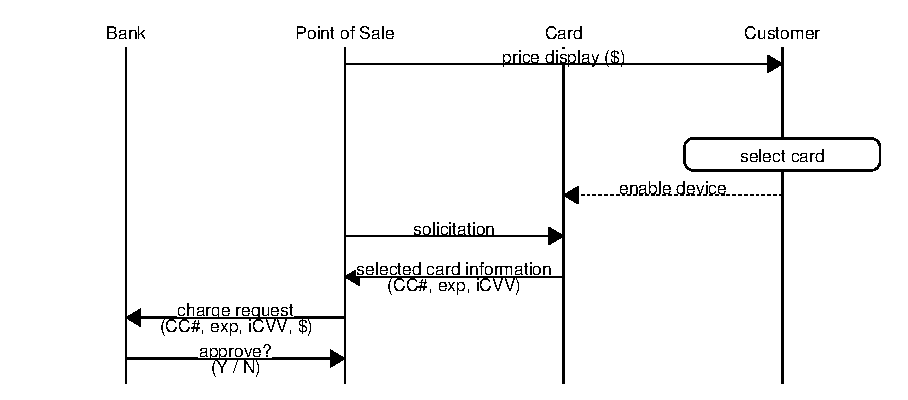
\includegraphics{img/wallet.eps}
  \label{fig:wallet}
\end{figure}

Electronic Wallets are advantageous for several reasons:
\begin{itemize}
\item Convenience: Electronic Wallets allow a customer to carry an essentially unlimited number of credit cards on their person without taking up extra space
\item Security: Electronic Wallets protect the customer from skimming and relay attacks,
    because Electronic Wallets are typically programmed not to respond to solicitations without customer consent.
    (Recall that physical credit cards will always respond to solicitation messages, regardless of the customer's intention.)
\item Interface: Electronic Wallets can provide a rich interface between the customer and the virtual credit card.
    This interface allows the customer to participate in the protocol.
\end{itemize}

Electronic Wallets will also be used in the Unlinkable CC Protocol, described in Chapter \ref{cha:unlinkable_design}.

\chapter{Protecting Customer Privacy: Unlinkability}
\label{cha:unlinkability}
Retailers today enjoy the ability to link multiple purchases to an individual customer by identifying multiple purchases made using the same credit card.
We argue that this is problematic from a privacy standpoint and present the prevention of this ability as a goal for a new contactless credit card protocol.
All CC Protocols discussed thus-far provide retailers with a property of credit card payments known as \emph{linkability}:
    retailers are able to link purchases made using the same card, in order to build purchasing profiles on their customers.
Customer purchasing profiles are valuable to retailers, because they allow for more targeted and effective marketing, and can be sold to interested third parties.

However, these purchasing profiles can be unpleasant to the customer from a privacy standpoint:
  purchasing habits can reveal sensitive and personal information.
Furthermore, a customer cannot opt-out of this profiling except by avoiding the use of credit cards.

Recall that in the Insecure CC Protocol described in Chapter \ref{cha:insecure} (and in widespread use today),
  the card discloses its card number, expiration date, and iCVV to the point of sale with every purchase.
Therefore, a retailer can link purchases simply by comparing card numbers of these purchases.
Any credit card protocol which gives the retailer access to the card number is linkable by definition.

With this in mind, we consider how to provide credit card payments with the converse property: \emph{unlinkability}.
Informally, if credit card purchases are unlinkable, then retailers cannot use them to construct purchasing profiles efficiently.

While giving the retailer access to the card number is sufficient to undermine unlinkability, it is not necessary.
For example, consider the Externally Secure CC Protocol, presented in Chapter \ref{cha:external} and shown in Figure \ref{fig:external_ccp_recall} for convenience.
In this protocol, the credit card number is not disclosed, and all authentication data (contained within the value \emph{T}) is indistinguishable from random to the retailer.
However, the charge token contains a constant card identifier \emph{ID}, required by the bank in order to identify the customer for which \emph{T} must be verified.
No two credit cards have the same \emph{ID}, and \emph{ID} does not change, so the retailer can simply link purchases using \emph{ID} instead of the card number.
More generally, if the protocol includes a message received by the retailer from which the customer's identity can be inferred, then the protocol cannot provide unlinkability.

\begin{figure}[h!]
  \caption{Externally Secure CC Protocol}
  \centering
    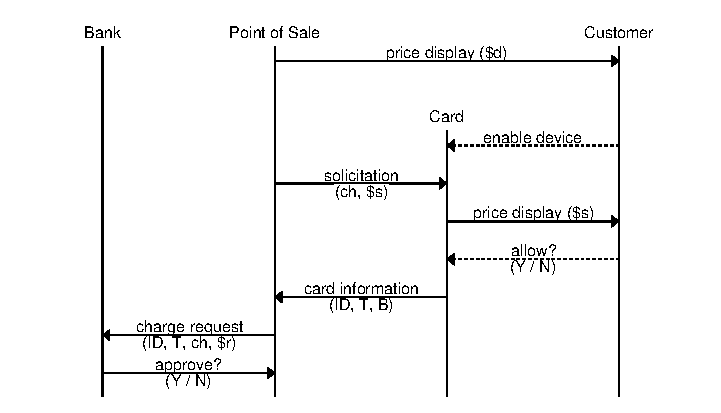
\includegraphics{img/secure_ccp.eps}
  \label{fig:external_ccp_recall}
\end{figure}


While we wish to conceal the customer's identity from the retailer, it must be disclosed to the bank in order for a charge to be processed.
As such, the problem reduces to one where we wish the contents of a message generated by a credit card (the message source)
  to be opaque to the point of sale (the carrier), but not to the bank (the final destination).
A natural approach to this problem is to use cryptography.

First let us consider symmetric cryptography, wherein the original sender (the credit card) and the final destination (the bank) share a secret key used for both encryption and decryption.
While symmetric cryptography can provide confidentiality of a message from the card to the bank, it cannot provide unlinkability.
This is because the message received by the bank must include some method for determining which of its customer's keys the bank should use to decrypt the message.
The retailer may then simply use this key identifier to link purchases.

Second, let us consider asymmetric (or ``public key'') cryptography,
  a system in which anybody (having access only to publicly available information) may encrypt a message that only the intended recipient may decrypt.
Indeed, it would not be difficult to construct a provably unlinkable payment protocol using asymmetric encryption:
a Card Information message may simply consist of the customer's credit card information, encrypted using the bank's public key.
The result is a Card Information message which is indistinguishable from random to the retailer.
The bank decrypts this message using its private key, reads the credit card information from the message body, and processes the payment.

Barring any other requirements, asymmetric cryptography provides sufficient primitives for constructing an unlinkable payment protocol.
However, asymmetric cryptography requires comparatively large (2048 bit) keys to be secure, and results in ciphertexts at least as long as the key.
For reasons to be discussed shortly in Section \ref{sec:goals-infrastructure}, we are limited to sending a single numeric 28-digit message to the point of sale.
As a result, using asymmetric cryptography in a secure manner is incompatible with our goals.

In conclusion, when constructing the Unlinkable CC Protocol, we need to define the Card Information message in such a way that it uniquely identifies the credit card to the bank,
  but where the entirety of the message is indistinguishable from random to the retailer,
  all while using at most 28 numeric digits.

\section{The Simple Unlinkable Protocol}
\label{sec:unlinkable-simple}

In considering a cryptographic approach to creating an Unlinkable Credit Card Protocol, let us first consider the simpler approach of using symmetric cryptography.
In a cryptographic scheme employing symetric cryptography,
    the original sender (the credit card) and the final destination (the bank) share a secret key used for both encryption and decryption.
While symmetric cryptography can provide confidentiality of a message from the card to the bank, it cannot provide unlinkability.
This is because the message received by the bank must include some method for determining which of its customer's keys the bank should use to decrypt the message.
The retailer may then simply use this key identifier to link purchases.

Let us next consider using asymetric (or ``public key'') cryptography,
  a system in which anybody (having access only to publicly available information) may encrypt a message that only the intended recipient may decrypt.
Asymetric cryptography allows the recipient to use a single key in order to decrypt messages originating from any party, sidestepping the key identifier issue above.

We thus present the Simple Unlinkable CC Protocol, employing asymetric encryption to maintain unlinkability.
This protocol is illustrated in Figure \ref{fig:simple-cpp}, and operates as follows:

\begin{figure}[h]
  \caption{Simple Unlinkable CC Protocol}
  \centering
    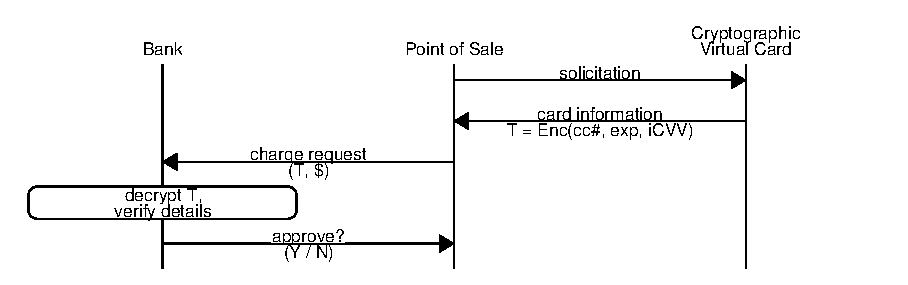
\includegraphics{img/simple-unlinkable-cpp.eps}
  \label{fig:simple-cpp}
\end{figure}

\begin{enumerate}
    \item The point of sale sends a Solicitation message to the customer's (virtual) credit card.
    \item The customer's card encrypts its credit card information (consiting of the credit card number, expiration date, and iCVV) using the bank's public key,
        and sends this data (along with the bank name) as a Card Information message.
    \item The point of sale receives the Card Information message, appends the price to charge, and sends this data to the bank indicated in the Card Information message.
    \item The bank decrypts the Card Information data to recover the customer's credit card number, expiration date, and iCVV.
        It then continues exactly as before in the Insecure CC Protocol described in Chapter \ref{cha:insecure}, responding to the point of sale with an Acceptance message.
\end{enumerate}

In this protocol, the Card Information message consists of an encrypted blob, and the bank name in cleartext.
The point of sale learns nothing about the customer, besides the name of the card's issuing bank.
As a result, this protocol is unlinkable.

Barring any other requirements, asymmetric cryptography provides sufficient primitives for constructing an unlinkable payment protocol.
However, asymmetric cryptography requires comparatively large (2048 bit) keys to be secure, and results in ciphertexts at least as long as the key.
For reasons to be discussed shortly in Section \ref{sec:goals-infrastructure}, our goals for an Unlinkable CC Protocol require much shorter message lengths.
As a result, using asymmetric cryptography in a secure manner is incompatible with our goals for a new Unlinkable CC Protocol.


\chapter{Additional Goals for the Unlinkable CC Protocol}
\label{cha:unlinkable_goals}

The Secure CC Protocol presented in Chapter \ref{cha:secure} is a significant improvement over the status quo (described in Chapter \ref{cha:insecure}).
However, the Secure CC Protocol neglects to provide two properties (in addition to Unlinkability) which we find desirable in a payment protocol:
  the ability to use existing point of sale infrastructure, and the ability to use any credit card.
We define and justify these goals, then use these three properties to guide the construction of a new protocol, which we call the Unlinkable CC Protocol.
This new protocol will maintain the benefits of the Secure CC Protocol, while simultaneously satisfying Unlinkability,
  the use of existing point of sale infrastructure, and the use of any credit card.

\section{Use Existing Point of Sale Infrastructure}
\label{sec:goals-infrastructure}

While constructing new and better protocols is an effective way to defend against attacks,
	requiring modification or updates to widely established infrastructure imposes a significant barrier to the adoption of this new protocol.
For example, in order to implement the Secure CC Protocol described in Chapter \ref{cha:secure}, every point of sale must be modified or replaced.
In order to sidestep this barrier, we consider the protocol in use today (the Insecure CC Protocol in Chapter \ref{cha:insecure}) from the perspective of a point of sale.

A point of sale may do rudimentary checks on the structure of the Card Information messages that it receives,
	but it relies on the bank in order to validate the data in these messages.
The Insecure CC Protocol, from the perspective of the point of sale, is illustrated in Figure \ref{fig:interface_pos} and operates as follows:

\begin{enumerate}
\item The point of sale issues a Solicitation message over the NFC channel.
	This message contains no payload of interest.
\item The point of sale receives a Card Information message over the NFC channel.
	This message consists of the following fields:
	\begin{itemize}
	\item a 16-digit card number
	\item a 4-digit expiration date
	\item an 8-digit iCVV
	\end{itemize}
	In practice, this is an opaque\footnote{
        There are some constraints on this value.
        For example, an expiration date of ``8321'' does not need to be verified by a bank to be declared invalid.
        Similarly, there are constraints on credit card numbers as well.
        These have little effect on our approach, so we ignore them for simplicity.
    }
    28-digit numeric value (16 + 4 + 8).
    This data is accompanied by the bank name.
\item After receiving the Card Information message,
	the point of sale issues a Charge Request message to the bank specified by the bank name field in the Card Information message.
	The Charge Request message consists of the card's credit card number, expiration date, iCVV, and the price to charge.
	In practice, this repeats the same 28-digit numeric value received in the Card Information message, accompanied by the price to charge.
\item Later, the point of sale receives an Approval message in response to the Charge Request message.
	The Approval message consists of the bank's decision on whether to accept the charge, as described in Section \ref{sec:insecure-design}.
\end{enumerate}

\begin{figure}[h!]
  \caption{Insecure CC Protocol, Point of Sale Behavior}
  \centering
    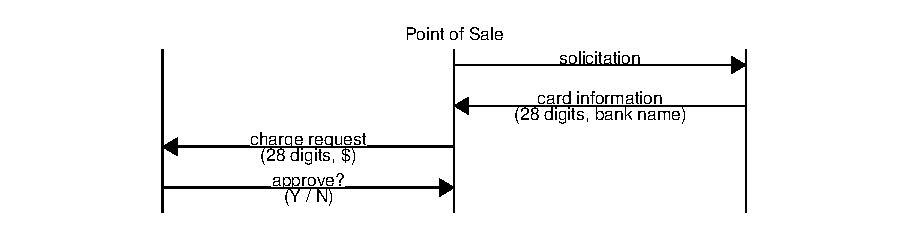
\includegraphics{img/interface_pos.eps}
  \label{fig:interface_pos}
\end{figure}

A key observation of the point of sale's behavior is that it consists of relaying data
	specified by the card to a destination \emph{also specified by the card}.
While the point of sale may interpret the 28-digit data content of the Card Information message as consisting of three fields describing a credit card,
	the customer may instead use these fields to encode an arbitrary 28-digit message, provided that the recipient of the Charge Request message decodes it accordingly.

We leverage this observation in the construction of the Unlinkable Wallet Protocol,
    conforming to existing point of sale behavior by using this 28-digit message as a carrier for the data we wish to transmit.
In so doing, we ensure that the point of sale in the Unlinkable Wallet Protocol remains identical to its counterpart in the Insecure CC Protocol.

\section{Use of Any Credit Card}
\label{sec:goals-anycard}

Few credit cards today support NFC transactions natively.
As a result, the majority of credit cards available to customers cannot generate valid iCVVs.
The Unlinkable CC Protocol should allow the use of any credit card, including those for which no valid iCVVs exist.

This matter is complicated by our goal of using existing point of sale infrastructure:
    current point of sale devices require an iCVV as part of an NFC Card Information message.
To get around this, we can leverage the architecture of credit cards themselves.

Each credit card is a collection of independent interfaces.
The common interfaces seen on credit cards today include:

\begin{itemize}
\item \textbf{visual}: the data which can be visually read from the card
\item \textbf{embossed}: the data physically embossed on the card
\item \textbf{magstripe}: the data encoded on the magnetic strip
\item \textbf{NFC}: the data and computation involved in contactless payments
\item \textbf{chip}: the data and computation involved in chip payments
\end{itemize}

These interfaces operate independently:
    a transaction involves the use of a single interface, as negotiated by the customer and the retailer.
The bank accepts a valid Charge Request over any interface supported by the credit card.
While some cards support a different set of interfaces than others, an important observation is that \emph{every} credit card supports the visual interface.

Making use of NFC communication is desirable for a new credit card protocol,
    because a smart phone supporting NFC communication enables the customer to send and receive arbitrary messages.
However, for a charge to be successful, the bank must receive a Charge Request pertaining to a \emph{non-NFC} interface,
    due to the lack of valid iCVVs associated with non-NFC credit cards.

These two seemingly contradictory requirements suggest the construction of a tunneled protocol:
    if we place an entity between the point of sale and the bank, this entity may receive an NFC Charge Request from the point of sale,
    convert it into a Charge Request of another interface (for example, the visual interface),
    and send this converted Charge Request to the bank.



\chapter{Design of the Unlinkable CC Protocol}
\label{cha:unlinkable_design}

In this chapter, we construct the Unlinkable CC Protocol, achieving our three primary goals:
supporting unlinkabile payments,
allowing the use of any credit card,
while using existing point of sale infrastructure.

We begin by making several strong assumptions.
In particular, we assume that:
\begin{itemize}
\item the retailer is not malicious,
\item the customer's Wallet Application is constantly connected to the Internet,
\item no messages between the point of sale and the bank are lost.
\end{itemize}
As we refine the protocol, we will erode these assumptions away to yield a secure and resilient protocol.

As foreshadowed in the previous chapter, this protocol will span multiple credit card interfaces.
In particular, our protocol design will make use of both the \emph{NFC}\footnote{
	When using the NFC interface, credit cards are authenticated via card number, expiration date, and iCVV.
} and the \emph{visual}\footnote{
	When using the visual interface, credit cards are authenticated via cardholder name, card number, and expiration date,
	optionally accompanied by the CVV2 (the 3-digit number on the back of the card) and/or billing address.
} interfaces.
As a result, message names in this chapter will identify the relevant interface where appropriate.

The Unlinkable CC Protocol will assume the exclusive use of Electronic Wallets.
This is necessary because when using a physical credit card, the customer has no control over the messages sent,
    and thus cannot alter the protocol.
Thus, the first step for a customer is to download the Wallet Application and register a credit card.

The card registration process is simple.
The customer enters the credit card details for the card he wishes to add into the Wallet Application.
These details consist of the cardholder name, card number, expiration date, and billing address.
The Wallet Application then sends this data in a Registration message to a new principal: the Wallet Server.
This Registration message is transmitted securely over the Internet.

The customer may then use any card registered through the Wallet Application to make unlinkable transactions.

\section{Basic Unlinkable Wallet Protocol}
\label{sec:unlinkable-design-1}

When the Wallet Server receives a Registration message,
    it stores the card information and associates a unique card identifier, denoted \emph{Ident}, with this record.
In the basic protocol, the Wallet Server responds to the Registration message with this identifier \emph{Ident}.
The Wallet Application stores this value securely, associating it with the credit card being registered.
The protocol, illustrated in Figure \ref{fig:unlinkable-1}, operates as follows:

\begin{figure}[h!]
  \caption{Basic Unlinkable Wallet Protocol}
  \centering
    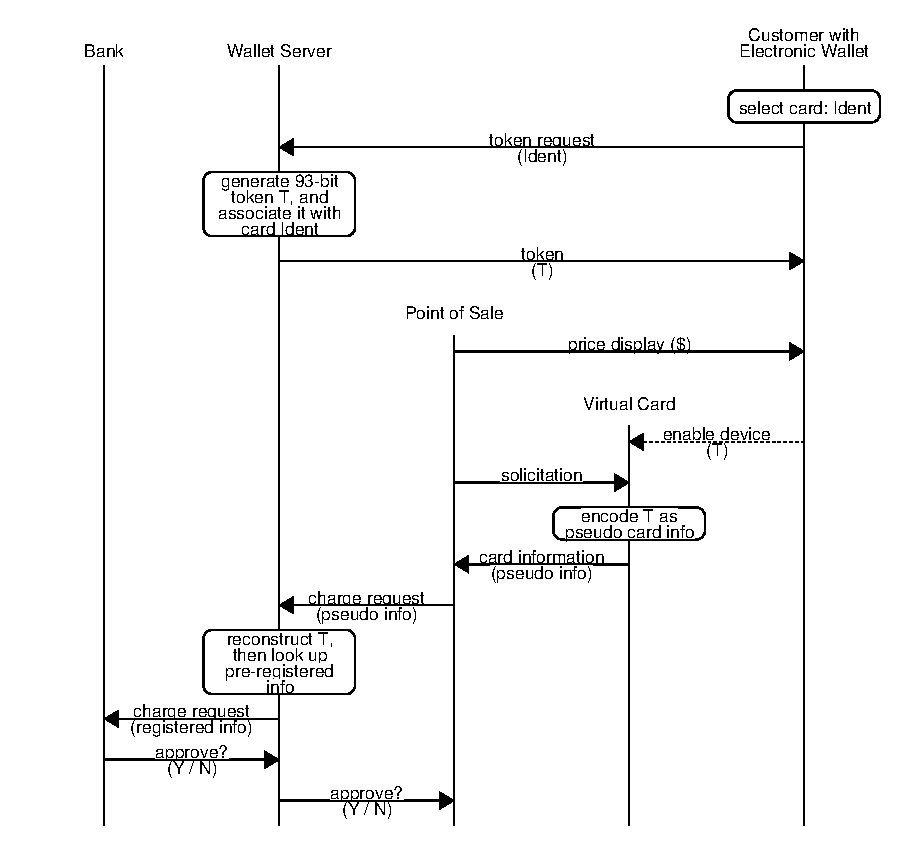
\includegraphics{img/unlinkable-1.eps}
  \label{fig:unlinkable-1}
\end{figure}

\begin{enumerate}

\item The customer selects a credit card in the Wallet Application.

\item The Wallet Application sends a Token Request message to the Wallet Server.
    This message consists of the card identifier \emph{Ident} associated with the selected card, and is sent securely over the Internet.
    Note that this message should be authenticated to prevent a customer from requesting a token to a different customer's card.

\item The Wallet Server then generates a random 93-bit token \emph{T} and associates it with the card identified by \emph{Ident}.
    The Wallet Server responds to the Wallet Application with a Token message containing \emph{T}.

\item The point of sale displays the price to charge (\val{\$}) on its screen.

\item The Wallet Application now enables the virtual credit card, initializing it with token \emph{T}.
    The virtual credit card begins listening for Solicitation messages.

\item The point of sale sends a Solicitation message to the virtual credit card over the NFC channel.

\item The virtual credit card converts token \emph{T} into a 28-digit number \emph{k}
    (note that 28 digits is sufficient to store a 93 bit value: $log_{10}(2^{93}) \approx 27.995$).
    It then responds with a Card Information message.
    This message has the following fields:
    \begin{itemize}
    \item \textbf{Pseudo Card number:} the first 16 digits of \emph{k}
    \item \textbf{Pseudo Expiration date:} the subsequent 4 digits of \emph{k}
    \item \textbf{Pseudo iCVV:} the remaining 8 digits of \emph{k}
    \item \textbf{Pseudo Bank name:} the Wallet Server
   	\end{itemize}

\item The point of sale constructs an Charge Request message from the (pseudo) card number, expiration date, iCVV, and the price it wishes to charge.
    This message is sent to the bank named in the Card Information message.
    As a result, the Charge Request message is directed to the Wallet Server and \emph{not} an actual bank.
    Note that from the perspective of the point of sale, the Wallet Server appears to be a bank like any other.

\item The Wallet Server reconstructs \emph{k} from the Charge Request message and computes the 93-bit token it represents.
    The Wallet Server then searches its database for this token, in order to identify the card used in this transaction.
    If the token is not found, the Wallet Server sends a ``declined'' Approval message to the point of sale and aborts the protocol.
    Otherwise, the stored card details are retrieved from the Wallet Server's database.
    The Wallet Server then invalidates the token and sends a \emph{visual} Charge Request to the card's bank with the following fields:
    \begin{itemize}
    \item Cardholder name
    \item Card number
    \item Expiration date
    \item Billing address
    \end{itemize}
    Note that unlike the Card Information message sent by the Wallet Application, this data reflects the actual credit card information,
        acquired by the Wallet Server during the card registration.

\item The bank receives the \emph{visual} Charge Request from the Wallet Server and processes this transaction as normal.
    It then responds to the Wallet Server with an Approval message indicating whether the charge has been accepted.

\item The Wallet Server forwards the bank's Approval message to the point of sale.
\end{enumerate}

Note that in this protocol, the Wallet Server has a dual role:
to the point of sale, the Wallet Server appears to be a bank, while to the bank, the Wallet Server appears to be a point of sale.

Note too that the Wallet Application needs to have a ready connection to the Internet.
Each transaction requires secure communication with the Wallet Server in order to receive the next token \emph{T}.
Should a connection to the Internet be unavailable to the Wallet Application,
    after using \emph{T}, the customer is unable to perform subsequent purchases with this virtual credit card until a Token Request exchange can take place.

This protocol is unlinkable,
    because the information received by the point of sale consists solely of a random value, accompanied by a bank name identifying the Wallet Server.
Any credit card can be used in this protocol,
    because the bank receives \emph{visual} Charge Request messages, and all credit cards support the visual interface.
Finally, this protocol uses existing infrastructure in that the behaviors of the point of sale and the bank are unchanged from those of the Insecure CC Protocol.

\section{Protecting against Malicious Retailers}
\label{unlinkable-design-2}

As before, upon card registration, the Wallet Server generates and stores a random token.
In this version of the protocol, this token is only 80 bits long.
The protocol then operates as follows:

\begin{enumerate}
    \item The point of sale displays the price to pay on its screen.
    \item The customer selects a credit card in the Wallet Application, and keys in the price to pay.
    \item The point of sale sends a Solicitation message to the Wallet Application over the NFC channel.
    \item The Wallet Application looks up the 80-bit token which was issued for the card selected by the customer.
        It then calculates a 13-bit price hash \emph{h\textsubscript{p} = H(token, price)}$|$\textsuperscript{13}.
        The Wallet Application then concatenates the token and price hash into a 93-bit value,
        and converts this value into an \emph{NFC} Card Information addressed to the point of sale using the same procedure as in the Basic Protocol.
    \item The Point of Sale receives the Card Information message, and constructs an \emph{NFC} Charge Request from it and the price it wishes to charge.
        This Charge Request message is sent to the Wallet Server as before.
    \item The Wallet Server reconstructs the 93-bit value from the Charge Request message, and splits it into the 80-bit token and 13-bit price hash.
\end{enumerate}
\section{Tolerating Lack of Internet Access}
\label{unlinkable-design-3}

Both the Basic Unlinkable Wallet Protocol described in Section \ref{sec:unlinkable-design-1}
    and the Secure Unlinkable Wallet Protocol described in Section \ref{sec:unlinkable-design-2}
    suffer from requiring access to the Internet when a transaction is being made.
Each transaction requires the virtual credit card to acquire a new token \emph{T} from the Wallet Server.
As such, temporary lack of Internet access
    (e.g. paying for parking in an underground garage, making purchases while in a foreign country, etc)
    significantly hampers the ability for customers to use their credit cards.
This can be alleviated somewhat by requesting multiple tokens at once, but remains a fundamental limitation of the protocols.

In this third protocol (termed simply the Unlinkable Wallet Protocol), we solve this problem by generating the single-use tokens within the Wallet Application.
Tokens are generated deterministically and using information available to both the Wallet Server and Wallet Application.
As a result, both the Wallet Application and Wallet Server are able to independently generate the same tokens for a given card without needing to communicate
    (over the Internet).
Communication between the Wallet Application and the Wallet Server is no longer necessary besides during card registration (and during the resolution of any synchronization problems).

As before, when the Wallet Server receives a Registration message, it stores the card information and associates a card identifier \emph{Ident} with this record.
It also generates a secret key \emph{SK} associated with this card.
In the Unlinkable Wallet Protocol, the Wallet Server responds to the Registration message with this identifier \emph{Ident} and the key \emph{SK}.
The Wallet Application stores these values securely, associating them with the credit card being registered.

Both the Wallet Application and the Wallet Server initialize a transaction counter for this card, and set it to zero.
In addition, the Wallet Server calculates the initial token \emph{T}, by calculating the keyed HMAC of the transaction counter (currently at 0), keyed with key \emph{SK}.
The Wallet Server stores this initial value of \emph{T} with the credit card record.
The protocol, illustrated in Figure \ref{fig:unlinkable-3}, operates as follows:

\begin{figure}[h!]
  \caption{Unlinkable Wallet Protocol}
  \centering
    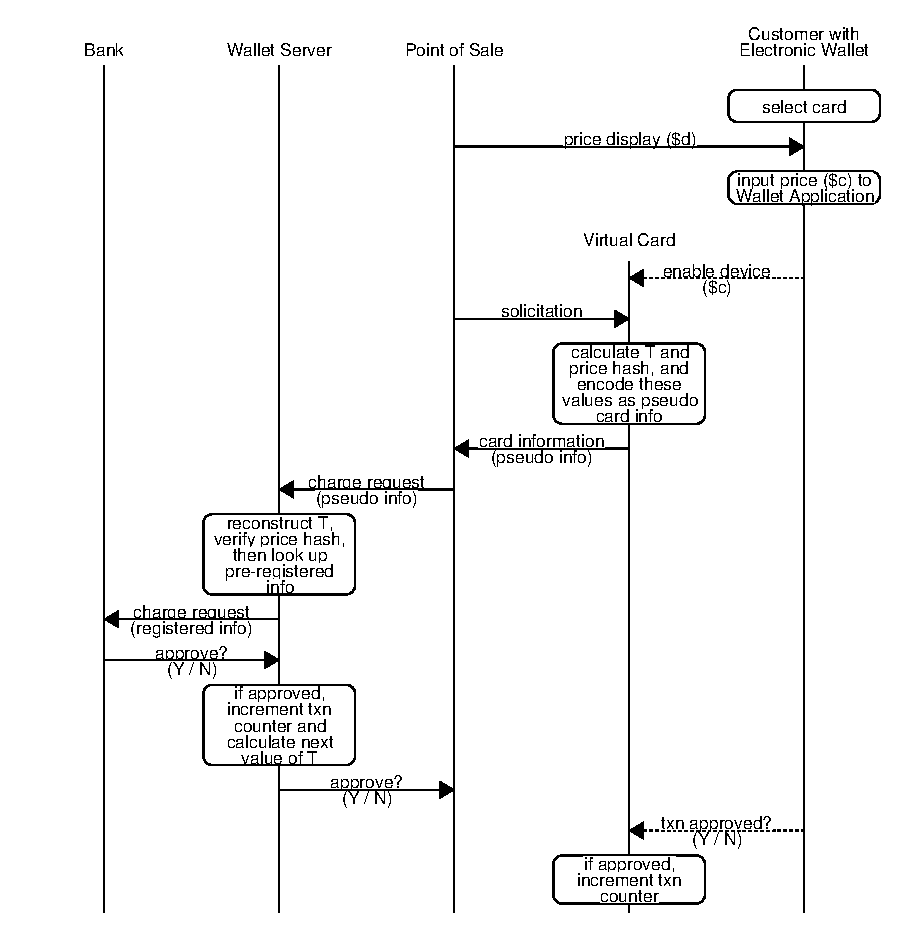
\includegraphics{img/unlinkable-3.eps}
  \label{fig:unlinkable-3}
\end{figure}

\begin{enumerate}
\item When the customer wishes to use a credit card, the customer selects a credit card in the Wallet Application.

\item The point of sale displays the price to charge (\val{\$d}) on its screen.

\item The customer enters the price to be charged (\val{\$c}) into the Wallet Application.

\item The Wallet Application now enables the virtual credit card, initializing it with price \val{\$c}.
    The virtual credit card begins listening for Solicitation messages.

\item The point of sale sends a Solicitation message to the virtual credit card over the NFC channel.

\item
    The virtual credit card calculates token \emph{T} by calculating the HMAC of the transaction counter keyed with the key \emph{SK}, and selecting the first 80 bits.
    The virtual credit card then proceeds as before.
    It calculates the price hash by combining \emph{T} with price \val{\$c},
        and calculating the HMAC of this value with key \emph{SK}, then selecting the first 13 bits.
    It then combines the 80-bit token \emph{T} with this 13-bit price hash to acquire a 93-bit value.
    Finally, it converts this 93-bit value into a 28-digit number \emph{k}, and responds with a pseudo Card Information message as before.

\item The point of sale constructs an Charge Request message from the (pseudo) Card number, Expiration date, iCVV, and the price it wishes to charge.
    This message is sent to the bank named in the Card Information message.
    As a result, the Charge Request message is directed to the Wallet Server and \emph{not} an actual bank.
    Note that from the perspective of the point of sale, the Wallet Server appears to be a bank like any other.

\item The Wallet Server reconstructs \emph{k} from the Charge Request message, and computes the 80-bit token and 13-bit price hash that it represents.
    The Wallet Server then searches its database for the token, to identify the card used in this transaction.
    If exactly one token is not found, the Wallet Server sends a ``declined'' Approval message to the point of sale, and aborts the protocol.
    Otherwise, the secret key \emph{SK} is retrieved from the Wallet Server's database, and the Wallet Server calculates its own version of the price hash
        using the price indicated by the point of sale in the Charge Request message.
    If the Wallet Server's price hash does not match the price hash in the Charge Request message,
        the Wallet Server sends a ``declined'' Approval message to the point of sale and aborts the protocol.
    Otherwise, the stored card information is retrieved from the Wallet Server's database.
    The Wallet Server sends a \emph{visual} Charge Request to the card's bank with the following fields:
    \begin{itemize}
    \item Cardholder name
    \item Card number
    \item Expiration date
    \item Billing address
    \end{itemize}
    Note that unlike the Card Information message sent by the Wallet Application, this data reflects the actual credit card information,
        acquired by the Wallet Server during the card registration.

\item The bank receives the \emph{visual} Charge Request from the Wallet Server, and processes this transaction as normal.
    The bank then responds to the Wallet Server with an Approval message indicating whether the charge has been accepted.

\item The Wallet Server examines the Approval message from the bank.
    If the charge was accepted, it increments the transaction counter associated with the virtual credit card, and recalculates the next expected value of \emph{T}.
    The Wallet Server then forwards the bank's Approval message to the point of sale.

\item The Wallet Application prompts the customer as to whether the charge was accepted by the bank.
    Note that the Approval message is not sent to the Wallet Application or virtual credit card as part of the protocol,
        and so the Wallet Application must rely on the customer to enter this data.
    If the charge was approved, then the virtual credit card increments its transaction counter.
\end{enumerate}

The Unlinkable Wallet Protocol is identical to the Secure Unlinkable Protocol,
    with the exception that the tokens \emph{T} are generated independently in both the Wallet Application and the Wallet Server.
As a result of this change, there are two potential failure cases which must be considered.

First, since the protocol relies on the customer manually maintaining the transaction counter within a virtual credit card,
    we must account for potential customer error.
If a customer fails to increment the transaction counter on a successful purchase (or incorrectly increments it on a failed purchase),
    then the Wallet Server and the virtual credit card will not agree on subsequent values of \emph{T}.
The transaction counter can be re-synchronized by way of an authenticated message exchange with the Wallet Server, sent securely over the Internet.
Customer error in maintaining a virtual credit card's internal transaction counter thus results in an inoperative virtual credit card
    until such a time as the Wallet Application regains temporary access to the Internet.

Second, since the Wallet Server can no longer exercise full control over token generation, we need to consider the possibility of token collisions.
A token collision occurs when two different virtual credit cards calculate the same token \emph{T} around the same time.
This occurs when \emph{H(SK\textsubscript{1}, txn\_ctr\textsubscript{1}) = H(SK\textsubscript{2}, txn\_ctr\textsubscript{2})}.
In this case, both virtual cards become inoperative until \emph{at least one} of the corresponding Wallet Applications regains access to the Internet
    and negotiates a new transaction counter\footnote{
    We refer to the value as a ``transaction counter'' because we increment it with every transaction,
        but there is no requirement that it reflect an accurate number of transactions.
    It need only be a value which (a) changes on every successful transaction, and
        (b) changes in such a way that both the Wallet Application and Wallet Server can independently agree on the new value.
    As such, resolution to a collision consists simply of incrementing the transaction counter of whichever card is first to reconnect to the Internet, and resynchronizing.
    }.
Note however that the probability of such a collision is negligibly small, and will be examined below in Chapter \ref{cha:analysis}.

\chapter{Analysis of the Unlinkable Wallet Protocol}
\label{cha:simulation}
The Unlinkable Wallet Protocol has several benefits tangible benefits, as described in the previous chapter.
However, collision mitigation strategies are inconvenient, and so it is important to understand the expected frequency of such events.
In this chapter, we analyze the features of the Unlinkable Wallet Protocol which make it attractive,
    as well as the statistical frequency of collisions.
\section{Security Analysis of the Protocol}
\label{sec:analysis}

The Unlinkable Wallet protocol is secure against malicious outsiders.
Simply by using an Electronic Wallet, the customer is protected from skimmers and relay attackers ``for free'',
    because the phone must be unlocked and ready to transmit in order to respond to a Solicitation message.
The Unlinkable Wallet Protocol provides protection against eavesdroppers and compromised points of sale,
    because each message consists of two single-use tokens which lose all value after the transaction takes place.

Due to the inclusion of the price validation hash (the last 13 bits of the 93-bit message),
    the Unlinkable Wallet Protocol defends against Malicious Retailers by binding the charge token to a price confirmed by the customer.

Furthermore, the Unlinkable Wallet Protocol provides the customer with the privacy property of \emph{Unlinkability} from the retailer.
In this protocol, retailers lose the ability to use credit card numbers as a method to correlate purchases and track customer purchasing profiles through purchase records.

In \cite{sccp} and \cite{ICDCN:15}, we considered Unlinkability an explicit non-goal:
  for deployment, the protocol required extensive cooperation from retailers who currently enjoy this property.
The Unlinkable Wallet Protocol requires no such cooperation from retailers or the payment industry,
    which means that bowing to retailers' wishes is not necessary.

Note that the information correlating an individual credit card to an individual purchase is not lost:
    it is now learned by the Wallet Server instead.

Indeed, the Wallet Server finds itself in a very privileged position:
    by inserting itself between retailers and banks, it appropriates knowledge from retailers regarding transaction correlation
    and appropriates knowledge from banks regarding transaction locations\footnote{
This appears to be consistent with the operation of Electronic Wallet applications like Android Pay and Apple Wallet:
    Android Pay has announced partnerships with some banks,
    which results in your credit card's purchases through Android Pay continuing to earn rewards normally offered by your credit card
    (e.g. 5 points per dollar spent on gas, 3 points per dollar spent on groceries, etc.).
    This suggests that, lacking a partnership with Electronic Wallet providers, banks lose information on the nature and location of purchases.}.

Even so, the Unlinkable Wallet Protocol protects customer privacy
    by separating knowledge of itemized purchases and correlation between purchases.
It is potentially valuable for an entity to be able to answer the questions \emph{Where does the customer spend money? What does the customer spend money on?}

Currently, banks have complete information on where customers spend their money,
    and retailers have have complete information on what their customers spend money on (at that retailer).
The Unlinkable Wallet Protocol breaks part of this information away from both parties:
    all purchases appear to the bank as being made out to the Wallet Server, and
    all purchases appear to the retailer as being made by a unique credit card.

\subsection{Collision Analysis of the Protocol}
\label{sec:collisions_and_simulations}

Every transaction processed by the Wallet Server service updates a card's Account Hash to a new 80-bit value.
If at any time two cards possess the same Account Hash, the Wallet Server can no longer process purchases for either card,
    as a Charge Request message cannot uniquely identify a card.
While hash functions such as those in the SHA-2 family are collision resistant, this does not mean that collisions cannot occur.
Furthermore, truncating the Account Hash down to 80 bits greatly increases the probability of collisions.

We wrote a simulator to model Wallet Server behavior, in order to ensure that messages contained sufficient information for the protocol to succeed,
    and to monitor for collisions.
We seeded it with 10 million credit cards, and processed several million transactions.
During the simulation, no collisions were observed.

Modeling this behavior mathematically, we note that the Birthday Paradox plays a role in determining the number of credit cards that a database can contain before expecting a hash collision:
the expected number cards registered before observing a collision is approximately
$\sqrt{\frac{\pi}{2} \cdot 2^{80}} \approx 1.4 \cdot 10^{12}$.
However, registering a credit card is by definition an event in which the Wallet Application is connected to the Internet (and thus to the Wallet Server).
As such, collisions during registration are not a concern, as a differing seed or counter value can simply be chosen and synchronized between the Wallet and the Server.
As a result, provided that there are fewer than $2^{79}$ (approximately $6.04 * 10^{24}$) credit cards registered, card registration is computationally easy (expecting no more than two attempts) without causing a collision.

A credit card transaction is then modeled by selecting a single hash and replacing it.
In such a transaction, the Birthday Paradox is not relevant:
intuitively, updating Hash number 83 cannot cause Hashes 12 and 41 to collide.
As a result, given a database of $n$ Account Hashes, the expected number of transactions before a collision occurs is
$\frac{2^{80}}{n}$.
Using the 10 million cards from our simulation, this implies that the expected number of transactions before a collision occurs is
$\frac{2^{80}}{10,000,000} \approx 1.2 \cdot 10 ^ {17}$, or approximately 120 million billion transactions.
It is thus hardly surprising that no collisions were observed in simulation.

As such, the inconvenience of rendering both cards inoperative until at least one of them reconnects to the Internet is not particularly onerous.

\chapter{Concluding Remarks and Future Work}
\label{cha:conclusion}
\todo{conclusion etc.}

\bibliographystyle{plain}
\bibliography{dissertation}
\index{Bibliography@\emph{Bibliography}}

\printindex

\begin{vita}
Oliver Christopher Jensen was born in Oxshot, England in 1987, and moved to Geneva, Switzerland before beginning school.
After graduating from the International School of Geneva in 2005 with an International Baccalaureate,
    he attended Colgate University in Hamilton, New York.
While at Colgate University, he worked on protocol research with Prof. Vijay Ramachandran,
    earning High Honors in Computer Science for his senior thesis on traceroute data integrity and route concealment.
He graduated in 2009 with a Bachelors of Arts in Mathematics and Computer Science.

Joining the University of Texas at Austin Computer Science Ph.D. program in 2010,
    Oliver focused his research on subjects relating to security and privacy.
Discovering a love for teaching, he taught an upper-division class on security and privacy in networked systems between 2014 and 2017.
Oliver was awarded a Masters of Computer Science with a minor in Electrical Engineering in December of 2013,
    and a Ph.D. of Computer Science in May of 2017.
\end{vita}

\end{document}
